
%%Packages import
\documentclass[a4paper, noexaminfo,oneside]{sapthesis}
\usepackage{microtype}
\usepackage[english]{babel}
\usepackage[utf8]{inputenc}
\usepackage[T1]{fontenc}
\usepackage{imakeidx}
\usepackage[acronym]{glossaries}
\captionsetup{labelsep=quad}
\usepackage{array}
\usepackage{ragged2e}
\usepackage[table]{xcolor}

\definecolor{citegreen}{RGB}{0, 128, 0} 
\definecolor{citeblack}{RGB}{0, 0, 0} 


\usepackage[colorlinks=true, citecolor=citegreen, linkcolor=black, urlcolor=black, filecolor=black]{hyperref}
% \usepackage[colorlinks=true, citecolor=citeblack, linkcolor=black, urlcolor=black, filecolor=black]{hyperref}
\usepackage{blindtext}
\usepackage{comment}
\usepackage{color,soul}
\usepackage{amsmath}
\usepackage{slashed}
\usepackage{amssymb}
\usepackage{wrapfig}
\usepackage{graphicx}
\usepackage{subcaption}
\usepackage{multirow}
\usepackage{booktabs}
% \usepackage{eso-pic}


\usepackage{pifont}
\newcommand{\xmark}{\ding{55}}

\usepackage[linguistics]{forest} 


\newcommand*{\belowrulesepcolor}[1]{% 
  \noalign{% 
  \kern-\belowrulesep \begingroup \color{#1}% 
  \hrule height\belowrulesep \endgroup }%
}
\newcommand*{\aboverulesepcolor}[1]{% 
  \noalign{%
  \begingroup \color{#1}% 
  \hrule height\aboverulesep \endgroup \kern-\aboverulesep }%
}

\usepackage[sort&compress,numbers]{natbib}
\bibliographystyle{unsrtnat}
\setcitestyle{lower,open={[},close={]}}

% \providecommand{\customexaminerlabel}{}

%%%%%%%%%%%%%%%%%%%%%%%%%%%%%%%%%%%%%%%%%%%%%%%%%%%%%
%%Main Settings
\hypersetup{pdftitle={Search for New Physics with Anomaly Detection approach at the LHC}, pdfauthor={Nome Cognome}}
\title{Search for New Physics in anomalous jets\\ using jet substructures with the ATLAS detector and LHC Run 3 data}
\author{Valerio Tinari}
\IDnumber{1998628}
\course{Master's Degree in Physics}
\courseorganizer{Facoltà di Scienze Matematiche, Fisiche e Naturali }
\AcademicYear{2025/2026}
\advisor{Prof. Stefano Giagu  }
\customadvisorlabel{Advisor}
\coadvisor{Dr. Valerio Ippolito \\Dr. Giuliano Gustavino}
\customcoadvisorlabel{Co-Advisors}
%\director{Dott.  Nome Cognome}
\authoremail{tinari.1998628@studenti.uniroma1.it}
\copyyear{2026}

\thesistype{Master's Thesis}

% \examdate{28/10/2026}
% \examiner{}

\makeindex

% \includeonly{Cap_1,Cap_2,Cap_3,Cap_4,Cap_5}
\newcommand{\Fig}[1]{[{\footnotesize \texttt{Fig.#1}}]}
\newcommand{\citfig}[1]{\ap{\scriptsize\textrm{(\textit{F#1})}}}

%%%%%%%%%%%%%%%%%%%%%%%%%%%%%%%%%%%%%%%%%%%%%%%%%%%%%%%%%%%%%%
%%Document
\begin{document}

\frontmatter
\maketitle
\dedication{"Te ne sei accorto, sì\\
Che passi tutto il giorno a disegnare\\
Quella barchetta ferma in mezzo al mare\\
E non ti butti mai"\\[1em]
\textit{Brunori Sas} - \textit{La Verità}}


\newpage
\thispagestyle{empty}
\mbox{} 
\newpage
\mainmatter
\phantomsection
\chapter*{Abstract}

This thesis implements the Anomaly Detection technique, a model-agnostic Machine Learning approach, to search for New Physics Beyond the Standard Model in fully hadronic final states with large-radius jets in the ATLAS experiment. 
The study focuses on four resonant BSM benchmark signals, among which Dark Jets and Heavy Vector Triplets, for different mass hypotheses of the resonant particles in the range between 2 TeV and 6 TeV. 
The background to those signals is dominated by QCD multi-jet production, with additional contributions from $t \bar{t}\rightarrow W^+W^-b\bar{b}$, $Z(\rightarrow qq) + jets$ and $W(\rightarrow qq) + jets$.
A Graph Neural Network is trained in an unbiased way on single jets from a Monte Carlo (MC) multi-jet sample simulating ATLAS Run-3 data, to compute the Anomaly Score (AS) of each jet.
The statistical analysis on the di-jet invariant mass $m_{JJ}$ distribution started with the definition of Working Points on the AS distribution, to achieve background rejection rates from 20\% to 99.9\%, values tested to investigate the minimum amount of background to discard in order to enhance the signals. 
After a careful optimization and validation of the parameteric modelling of the signal and background distributions via spurious signal tests and signal injection tests, the expected upper limits at 95\% Confidence Level on the cross section of the signals using binned maximum likelihood fits are derived using the CLs method.
A complete validation was realized performing sensitivity studies to derive an estimation of the sensitivity of the analysis with the partial and full ATLAS Run 3 dataset.
The results of the study show that an event selection based on the AS is competitive with the canonincal model-dependent seletions, presenting a possible improvement in the sensitivity to BSM signals, especially for the HVT benchmark signal in the VzWW process.





\newpage
\thispagestyle{empty}
\mbox{} 
\newpage
\mainmatter
\tableofcontents

\newpage
\thispagestyle{empty}
\mbox{} 
\newpage
\mainmatter
\phantomsection
\chapter*{Introduction}
\addcontentsline{toc}{chapter}{Introduction}

It was 4 July 2012 when Joseph Incandela, CMS spokesperson, affirmed: "\textit{They combine to give us a combined significance of five standard deviations}". With these exact words, he announced, confirmed by ATLAS spokesperson Fabiola Gianotti a few minutes later, the first observation of the Higgs boson \cite{HiggsDiscoveryATLAS,HiggsDiscoveryCMS}, which completed the Standard Model (SM) framework. Fourteen years later, no comparable discovery has followed within the SM paradigm at collider experiments, strengthening the hypothesis that it is the most complete and well-tested description of nature.\\
In reality, the SM probably is not as complete as it appears. In fact, there are many phenomena not included in the framework but confirmed by astrophysical and cosmological observations: among these, we can find the neutrino mass measurement, Dark Matter \cite{DM_Garrett} and baryon asymmetry. All these processes fall into the category of New Physics (NP) Beyond the Standard Model (BSM). They have been hunted by ATLAS and CMS experiments using traditional data analysis techniques, targeting specific theoretical models but, unfortunately, nothing has been observed yet and only upper limits on production cross-sections were set. There are many reasons for this unexpected outcome: wrong physical model for experiments, wrong triggering while selecting data, or deviations too small to be observed through normal techniques.\\
A possible solution to some of these issues could be Anomaly Detection (AD), that is the search for data deviating from what is already known. In our field of interest, Particle Physics, we apply this method to look for anomalies (signal data), deviating from well known reacting and decaying particles (background data). The strength of this method lies in its model agnostic nature, meaning that it does not rely on a specific theoretical model to analyse data. This allows us to explore a more vast range of events, increasing the background rejection efficiency, giving us a first hint of the region where to look more in depth for New Physics with precise data analysis techniques. In this process, unsupervised Machine Learning (ML) helps speeding up everything.\\
This thesis investigates whether such an unsupervised approach can be applied to a concrete search. Using ATLAS official Monte Carlo (MC) samples simulating the ATLAS detector during Run-3, a search for BSM resonant signals decaying into hadronic final states with large-radius jets (used to probe boosted resonance topologies) has been conducted, preparing the necessary tools to finalise the analysis on real ATLAS data. Leveraging the Anomaly Score (AS) distributions computed by a Graph Neural Network (GNN) for each jet, the analysis strategy was defined, starting with the definition of Working Points (WPs), thresholds on the AS distribution corresponding to a given background rejection fraction. A crucial part of the strategy was determining the correct modelling function for the background and signals di-jet invariant mass ($m_{JJ}$) distribution. After tuning and validating a Double-Sided Crystal Ball (DSCB) function to model the signals and a 5-parameter function for the background distribution, fits to the MC samples were executed, deriving the expected
upper limits at 95\% Confidence Level on $m_{JJ}$ using the CLs method, at different AS WPs. The study on MC samples was concluded and fully validated by performing sensitivity studies based on a binned maximum likelihood fit to the di-jet invariant mass distribution.\\
The thesis is structured as follows. In Chapter \ref{chap:SM_BSM} the Standard Model is presented, together with theories of Physics beyond it. 
The LHC collider and the ATLAS experiment are discussed in Chapter \ref{chap:LHCAtlas}, followed, in Chapter \ref{chap:Reco}, by the description of the techniques used within the ATLAS collaboration to reconstruct and identify the particles produced in the collisions.
Chapter \ref{chap:AD} presents the Anomaly Detection approach.
Chapter \ref{chap:ADJJ} presents the analysis conducted during this study and its results.
Finally, conclusions are drawn in Chapter \ref{chap:concl}.\\[1em]
The original contributions of this thesis are related to the validation of the GNN training and the implementation of the analysis strategy on the MC samples.
In particular, after determing that a jet-level AS is a good choice for the analysis, given the reduced correlation with kinematic variables, the WPs were computed, defining an event selection strategy based on the AS distribution.
Major efforts were spent in the development of the procedures to model and fit the $m_{JJ}$ distribution, both for the background and the signals, through rigorous validation tests.
The results of these studies were instrumental in sensitivity studies and in the derivation of the expected upper limits on the production cross-section of the signals.
These studies were followed by the definition of a proposal for the analysis strategy to be applied on real data collected by ATLAS during Run 3.
All the steps and results of this work are presented in Chapter \ref{chap:ADJJ}.
 




\chapter{(Beyond) The Standard Model } \label{chap:SM_BSM}
The Standard Model (SM) of Particle Physics is a relativistic Quantum Field Theory (QFT) describing three out of four fundamental interactions, strong, weak and electromagnetic (EM), and the behavior of elementray particles under them.
For a long time it was attempted to merge the fourth fundamental interaction, gravity, with the SM framework, but those attempts have not been validated yet by experimental observations. Nevertheless, for our purposes, gravity does not play a significant role since the energy scales involved in the processes at a collider experiment, as the LHC, are much lower than the Planck scale, where gravitational effects become relevant.\\
What is remarkable about the SM is that it is a very well tested theory, with predictions confirmed by experimental observations with a very high precision. The discovery of the Higgs boson in 2012 at the LHC, which completed the SM framework, is a clear example of this.\\
Despite the success of the SM, there are many phenomena that are not explained by it, but are confirmed by astrophysical and cosmological observations, opening the road for Physics Beyond the Standard Model.\\
This chapter presentes a brief overview of the SM, highlighting its major features. In addition, hints for Physics Beyond it are exposed.

\section{An overview of the Standard Model} \label{sec:SM_BSM/SM}
The fundamental constituents of Universe are precisely described by the SM. They are called elementary particles, which are mathematically described as quantum fields $\psi(x)$ and their dynamics is modelled by Lagrangian densities $\mathcal{L}(\psi, \partial_{\mu}\psi)$ \cite{Peskin_QFT}. 

\begin{figure}[ht!]
    \centering
    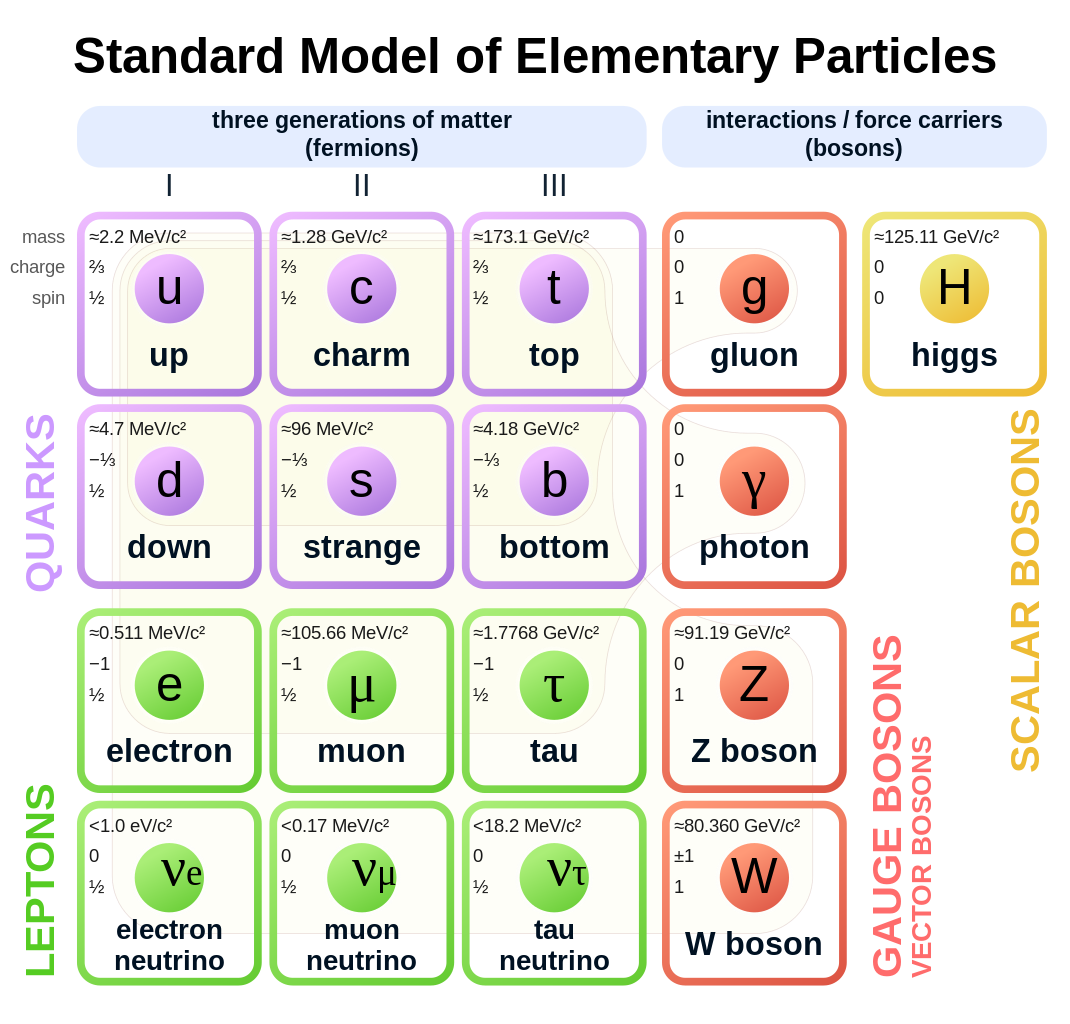
\includegraphics[width=3 in]{Images/Chap1/SM_framework.png}
    \caption{The SM framework. Figure from Ref. \cite{SM_wiki}.}
    \label{fig:SM_BSM/SM/SM_framework}
\end{figure}

\noindent Such particles can be graphically pictured as presented in Fig. \ref{fig:SM_BSM/SM/SM_framework}. 
They are divided into two fundamental classes based on their spin quantum number. The first class is composed by \textit{fermions}, which cover the first three column of Fig. \ref{fig:SM_BSM/SM/SM_framework} and are organised in three \textit{generations} of increasing proper mass; they have spin 1/2 and constitute \textit{matter}. The second class is those of \textit{bosons}, with integer spin, which \textit{mediate} fundamental interactions and generate mass.\\
Fermions are further classified into two distinct categories depending on their participation in the strong interaction. The first category is relative to \textit{quarks}. They carry \textit{colour charge} (red, green, blue), making them triplets under $SU(3)$ and therefore interact via all fundamental forces, among which the strong one.
Quarks exist in six flavors, organized into three generations of weak SU(2) doublets:
\begin{equation}\label{eq:SM_BSM/SM/quarks}
    \begin{pmatrix} u \\ d \end{pmatrix}, \quad 
    \begin{pmatrix} c \\ s \end{pmatrix}, \quad 
    \begin{pmatrix} t \\ b \end{pmatrix}
\end{equation}
Quarks carry a fractional electromagnetic charge: the \textit{up-type} ones ($u, c, t$) have a charge of $+2/3$, while the \textit{down-type} ones ($d, s, b$) carry a $-1/3$ charge.\\
The second category of fermions is associated to \textit{leptons}; they are six and similarly grouped into three generations:
\begin{equation}\label{eq:SM_BSM/SM/leptons}
    \begin{pmatrix} e^- \\ \nu_e \end{pmatrix}, \quad 
    \begin{pmatrix} \mu^- \\ \nu_\mu \end{pmatrix}, \quad 
    \begin{pmatrix} \tau^- \\ \nu_\tau \end{pmatrix}
\end{equation}
The charged leptons ($e^-, \mu^-, \tau^-$) carry an electric charge of $-1$ and interact via electromagnetic and weak forces. Neutrinos ($\nu_e, \nu_\mu, \nu_\tau$) are electrically neutral and interact exclusively via the weak force.\\
Both quarks and charged leptons, have their own anti-particles, which have the same mass of the matter components but opposite quantum numbers. Regarding neutrinos, it is still debated and to be proved whether they have a distinct anti-particles or they are Majorana fermions, being their own anti-particles.\\
The second class of particles is associated to mediatiors and mass. Spin 1 vector bosons, known as \textit{gauge bosons}, are the mediators of three of the fundamental interactions, which arise naturally from the requirement of local gauge invariance. Among those fields we find the 8 massless gluons $g$ mediating the strong interaction, the massless photon $\gamma$ is associated to electromagnetic interaction and 3 massive vector bosons, $W^\pm \text{ and } Z^0$, with masses $m_W=80.36\text{ GeV}$, $m_Z=91.19\text{ GeV}$, mediating the weak interaction.\\
In conclusion, a spin 0 scalar particle, the \textit{Higgs boson} $H$, with a mass $m_H = 125.13\text{ GeV}$, completes the particle spectrum, arising as a physical state from the spontaneous breaking of electroweak symmetry.\\

%-------------------------------------------------%
\noindent The SM is a gauge theory, meaning that the Lagrangian is invariant under local transformations of the fields. The Lagrangian density describing the SM dynamics is:

\begin{equation}\label{eq:SM_BSM/SM/SM_Lag}
\mathcal{L}_{\text{SM}} = -\frac{1}{4} F_{\mu\nu} F^{\mu\nu} - i\bar{\psi} \gamma_\mu D^\mu \psi + (D_\mu \phi)^\dagger (D^\mu \phi) - V(\phi) + \bar{\psi}_i y_{ij} \psi_j \phi + h.c.,
\end{equation}

\noindent The gauge group of the SM, under which such lagrangian is invariant, is a non-abelian symmetry group defined as:

\begin{equation}
    SU(3)_C \otimes SU(2)_L \otimes U(1)_Y
\end{equation}
\noindent where $SU(3)_C$ describes the strong interaction via Quantum Chromodynamics (QCD) with subscript \textit{C} standing for colour, and $SU(2)_L \otimes U(1)_Y$ represents the unified electroweak (EW) interaction, with \textit{L} associated to the left component of fermions and \textit{Y} to hypercharge.\\
The terms of the equation \ref{eq:SM_BSM/SM/SM_Lag} above are presented in detail in the following sections.

%-------------------------------------------------------------------------------
\subsection{Quantum Electrodynamics}\label{subsec:SM_BSM/SM/QED}
The first and simplest gauge theory within the SM framework is Quantum Electrodynamics (QED). It describes the electromagnetic interactions between a charged massive fermion, with mass \textit{m} and represented by a field $\psi(x)$, and the photon, the massless gauge boson represented by the vector field $A_\mu$.
Using the Lagrangian formalism \cite{Feynman_QFT}, QED is constructed starting from the free Dirac Lagrangian for a massive fermion \cite{pich_QED_EW}:

\begin{equation}\label{eq:SM_BSM/QED/Dirac_L}
    \mathcal{L}_\text{Dirac} = \bar{\psi} (i\gamma^\mu \partial_\mu - m) \psi
\end{equation}

\noindent In the equation above, $\bar{\psi} = \psi^\dagger \gamma^0$ is the Dirac adjoint of the field $\psi$ and $\gamma^\mu$ are the Dirac matrices derived from Pauli matrices $\sigma_i$ ($i$ =1,2,3 and $\mu$=0,1,2,3): 

\begin{equation}\label{eq:SM_BSM/QED/PauliMatrix}
\gamma^0 = \begin{pmatrix} 0 & \mathbb{I} \\ \mathbb{I} & 0 \end{pmatrix}, \qquad
\gamma^i = \begin{pmatrix} 0 & \sigma_i \\ -\sigma_i & 0 \end{pmatrix}
\end{equation}

\noindent The Dirac Lagrangian \ref{eq:SM_BSM/QED/Dirac_L} is invariant under a global $U(1)$ phase transformation $\psi(x) \to e^{i e \alpha} \psi(x)$, with $e$ the electric charge of the fermion and $\alpha$ a constant phase.
Such invariance is not preserved under a local $U(1)$ phase transformation $\psi(x) \to e^{i e \alpha(x)} \psi(x)$, where $\alpha(x)$ is a space-time dependent phase. In order to preserve the invariance, the partial derivative $\partial_\mu$ is replaced by the covariant derivative $D_\mu$:

\begin{equation}\label{eq:SM_BSM/QED/cov_der}
    D_\mu = \partial_\mu + i e A_\mu(x)
\end{equation}
where $A_\mu(x)$ is a vector gauge field representing the photon field, which transforms as $A_\mu(x) \to A_\mu(x) - \partial_\mu \alpha(x)$. Including the gauge-invariant kinetic term to take into account for the new field $A_\mu$, we derive the full QED Lagrangian:

\begin{equation}\label{eq:SM_BSM/QED/QED_L}
    \mathcal{L}_\text{QED} = \bar{\psi} (i\gamma^\mu D_\mu - m) \psi - \frac{1}{4} F_{\mu\nu} F^{\mu\nu}
\end{equation}
where $F_{\mu\nu} = \partial_\mu A_\nu - \partial_\nu A_\mu$ is the electromagnetic field strength tensor. The interaction term $-e \bar{\psi} \gamma^\mu \psi A_\mu$ rules the coupling of charged fermions to photons with a strength proportional to the electric charge $e$.


\subsection{Quantum Chromodynamics}\label{subsec:SM_BSM/SM/QCD}
\subsection{Electroweak model}\label{subsec:SM_BSM/SM/EW}

\section{Hints of Physics Beyond the Standard Model}\label{sec:SM_BSM/BSM}


/////////////////////////////////////////// \\

%-------------------------------------------------------------------------------


%-------------------------------------------------------------------------------
\subsection{Quantum Chromodynamics}
\label{subsec:qcd}

Quantum Chromodynamics (QCD) is the non-Abelian gauge theory describing the strong force acting between color-charged quarks and gluons. QCD is based on the local $SU(3)_C$ gauge symmetry, where $C$ represents the triplet color degree of freedom (red, green, blue). The Lagrangian for $N_f$ quark flavors is given by:
\begin{equation}
    \mathcal{L}_\text{QCD} = \sum_{f} \bar{q}_f^a \left( i \gamma^\mu (D_\mu)_{ab} - m_f \delta_{ab} \right) q_f^b - \frac{1}{4} G_{\mu\nu}^A G^{A, \mu\nu}
\end{equation}
where $q_f^a$ represents a quark field of flavor $f$ and color index $a \in \{1, 2, 3\}$. The gauge-covariant derivative is defined as:
\begin{equation}
    (D_\mu)_{ab} = \partial_\mu \delta_{ab} - i g_s T^A_{ab} A_\mu^A
\end{equation}
where $g_s$ is the strong coupling constant, $A_\mu^A$ ($A = 1, \dots, 8$) are the eight gluon vector fields, and $T^A = \frac{1}{2} \lambda^A$ are the $SU(3)$ generators expressed via the Gell-Mann matrices satisfying $[T^A, T^B] = i f^{ABC} T^C$.

The non-Abelian structure gives rise to the field strength tensor:
\begin{equation}
    G_{\mu\nu}^A = \partial_\mu A_\nu^A - \partial_\nu A_\mu^A + g_s f^{ABC} A_\mu^B A_\nu^C
\end{equation}
The presence of the non-linear structure constant term $f^{ABC}$ introduces triple and quadruple gluon self-interactions. This characteristic yields two defining physical properties of QCD:
\begin{enumerate}
    \item \textbf{Asymptotic Freedom:} At high energy scales (short distances), the running coupling constant $\alpha_s(Q^2) = \frac{g_s^2}{4\pi}$ decreases logarithmically, enabling accurate calculations via perturbative QCD (pQCD).
    \item \textbf{Color Confinement:} At low energy scales (long distances), $\alpha_s(Q^2)$ grows large. Colored particles cannot exist as isolated free states; they undergo fragmentation and hadronization, producing collimated sprays of energetic, neutral hadrons known as \textbf{jets}.
\end{enumerate}

%-------------------------------------------------------------------------------
\subsection{Electroweak Model}
\label{subsec:electroweak}

The unification of electromagnetic and weak interactions is realized through the Glashow-Weinberg-Salam (GWS) model, structured around the local gauge symmetry group $SU(2)_L \times U(1)_Y$. The left-handed fermion components transform as doublets under weak isospin $T$, whereas right-handed components transform as singlets:
\begin{equation}
    \Psi_L = \begin{pmatrix} \nu_{L} \\ e_L^- \end{pmatrix} \quad (T = 1/2, T_3 = \pm 1/2), \qquad e_R^- \quad (T = 0, T_3 = 0)
\end{equation}
Electric charge $Q$, weak isospin $T_3$, and weak hypercharge $Y$ are unified by the Gell-Mann-Nishijima relation:
\begin{equation}
    Q = T_3 + \frac{Y}{2}
\end{equation}

The gauge-covariant derivative introducing three $W_\mu^i$ ($i=1,2,3$) bosons for $SU(2)_L$ and one $B_\mu$ boson for $U(1)_Y$ is written as:
\begin{equation}
    D_\mu = \partial_\mu - i g T^i W_\mu^i - i g' \frac{Y}{2} B_\mu
\end{equation}

Spontaneous Symmetry Breaking (The Higgs Mechanism)
Unbroken $SU(2)_L \times U(1)_Y$ symmetry forbids mass terms for gauge bosons and fermions, as explicit mass terms violate local gauge invariance. Mass generation is accommodated via the Brout-Englert-Higgs mechanism by introducing a complex scalar doublet field $\Phi$:
\begin{equation}
    \Phi = \frac{1}{\sqrt{2}} \begin{pmatrix} \phi^+ \\ \phi^0 \end{pmatrix}, \quad \mathcal{V}(\Phi) = \mu^2 \Phi^\dagger \Phi + \lambda (\Phi^\dagger \Phi)^2 \quad (\mu^2 < 0, \lambda > 0)
\end{equation}
The scalar field acquires a non-zero vacuum expectation value (VEV) $v = \sqrt{-\mu^2/\lambda} \approx 246\text{ GeV}$, spontaneously breaking the symmetry:
\begin{equation}
    SU(2)_L \times U(1)_Y \xrightarrow{\text{SSB}} U(1)_\text{EM}
\end{equation}
Expanding $\Phi$ around its minimum in the unitary gauge transforms three degrees of freedom into longitudinal polarization states for the gauge physical bosons $W^\pm$ and $Z^0$:
\begin{equation}
    W_\mu^\pm = \frac{1}{\sqrt{2}}(W_\mu^1 \mp i W_\mu^2), \quad 
    \begin{pmatrix} Z_\mu \\ A_\mu \end{pmatrix} = \begin{pmatrix} \cos\theta_W & -\sin\theta_W \\ \sin\theta_W & \cos\theta_W \end{pmatrix} \begin{pmatrix} W_\mu^3 \\ B_\mu \end{pmatrix}
\end{equation}
where $\theta_W = \arctan(g'/g)$ is the weak mixing angle. The photon field $A_\mu$ remains massless, while gauge bosons acquire masses $m_W = \frac{1}{2} g v$ and $m_Z = \frac{1}{2} v \sqrt{g^2 + g'^2}$. Fermions acquire mass through gauge-invariant Yukawa couplings:
\begin{equation}
    \mathcal{L}_\text{Yukawa} = -y_f \bar{\Psi}_L \Phi f_R + \text{h.c.} \quad \implies \quad m_f = \frac{y_f v}{\sqrt{2}}
\end{equation}

%-------------------------------------------------------------------------------
\section{Hints of Physics Beyond the Standard Model}
\label{sec:bsm}

Despite the extraordinary predictive precision of the Standard Model—culminating in the discovery of the Higgs boson at the LHC in 2012~\cite{ATLAS:2012, CMS:2012}—it cannot be regarded as a complete theory of fundamental interactions. Unresolved theoretical open issues and physical phenomena observed in nature mandate the existence of Physics Beyond the Standard Model (BSM)~\cite{Garrett:2011}:

\begin{itemize}
    \item \textbf{Dark Matter:} Astrophysical and cosmological observations (galaxy rotation curves, gravitational lensing, cosmic microwave background) firmly establish that non-baryonic \textit{Dark Matter} comprises $\approx 26.8\%$ of the energy density of the Universe~\cite{Garrett:2011}. The SM offers no suitable stable, cold, weakly-interacting candidate particle~\cite{Garrett:2011}.
    
    \item \textbf{Neutrino Masses:} Oscillations observed in solar, atmospheric, and reactor neutrinos demonstrate that neutrinos possess non-zero masses, contrasting the strict masslessness assumed in the minimal SM structure.
    
    \item \textbf{Baryon Asymmetry:} The observable universe consists almost entirely of matter rather than antimatter~\cite{Garrett:2011}. The magnitude of $CP$ violation provided by the SM CKM matrix is insufficient to account for the observed cosmic matter-antimatter asymmetry~\cite{Garrett:2011}.
    
    \item \textbf{The Hierarchy Problem:} Quantum loop corrections to the scalar Higgs boson mass quadratic divergences yield corrections proportional to the Planck scale ($\Lambda_{\text{Planck}} \approx 10^{19}\text{ GeV}$). Maintaining $m_H \approx 125\text{ GeV}$ requires extreme, fine-tuned cancellations without a protective symmetry (such as Supersymmetry).
    
    \item \textbf{Quantum Gravity:} The Standard Model does not incorporate gravitational interactions. A quantum formulation of gravity compatible with General Relativity remains omitted at high energy scales.
\end{itemize}

These limitations motivate the search for new BSM resonance states and heavy new physics at collider experiments like the Large Hadron Collider (LHC)[cite: 9].
\chapter{The LHC and the ATLAS experiments} \label{chap:LHCAtlas}

The history of the European Organization for Nuclear Research (CERN) traces back to the post-WWII era, when European physicists, including Edoardo Amaldi, Niels Bohr and Pierre Auger, promoted a collaborative international laboratory dedicated to fundamental science. CERN was established in September 1954 and today it hosts the world's largest and most energetic accelerator complex, centered around the Large Hadron Collider (LHC).\\
In the following, after a description of the LHC machine, the discussion covers the architecture of the ATLAS (A Toroidal LHC ApparatuS) detector, one of the four major experiments at CERN, including its main sub-systems and simulation procedures. A special focus is given to the proton-proton collision dataset collected by ATLAS at a center-of-mass energy of 13.6 TeV during LHC Run 3, which forms the basis for this study.


%-------------------------------------------------------------------------------
%-------------------------------------------------------------------------------

\section{The LHC} \label{sec:LHCAtlas/LHC}

\begin{figure}[ht!]
    \centering
    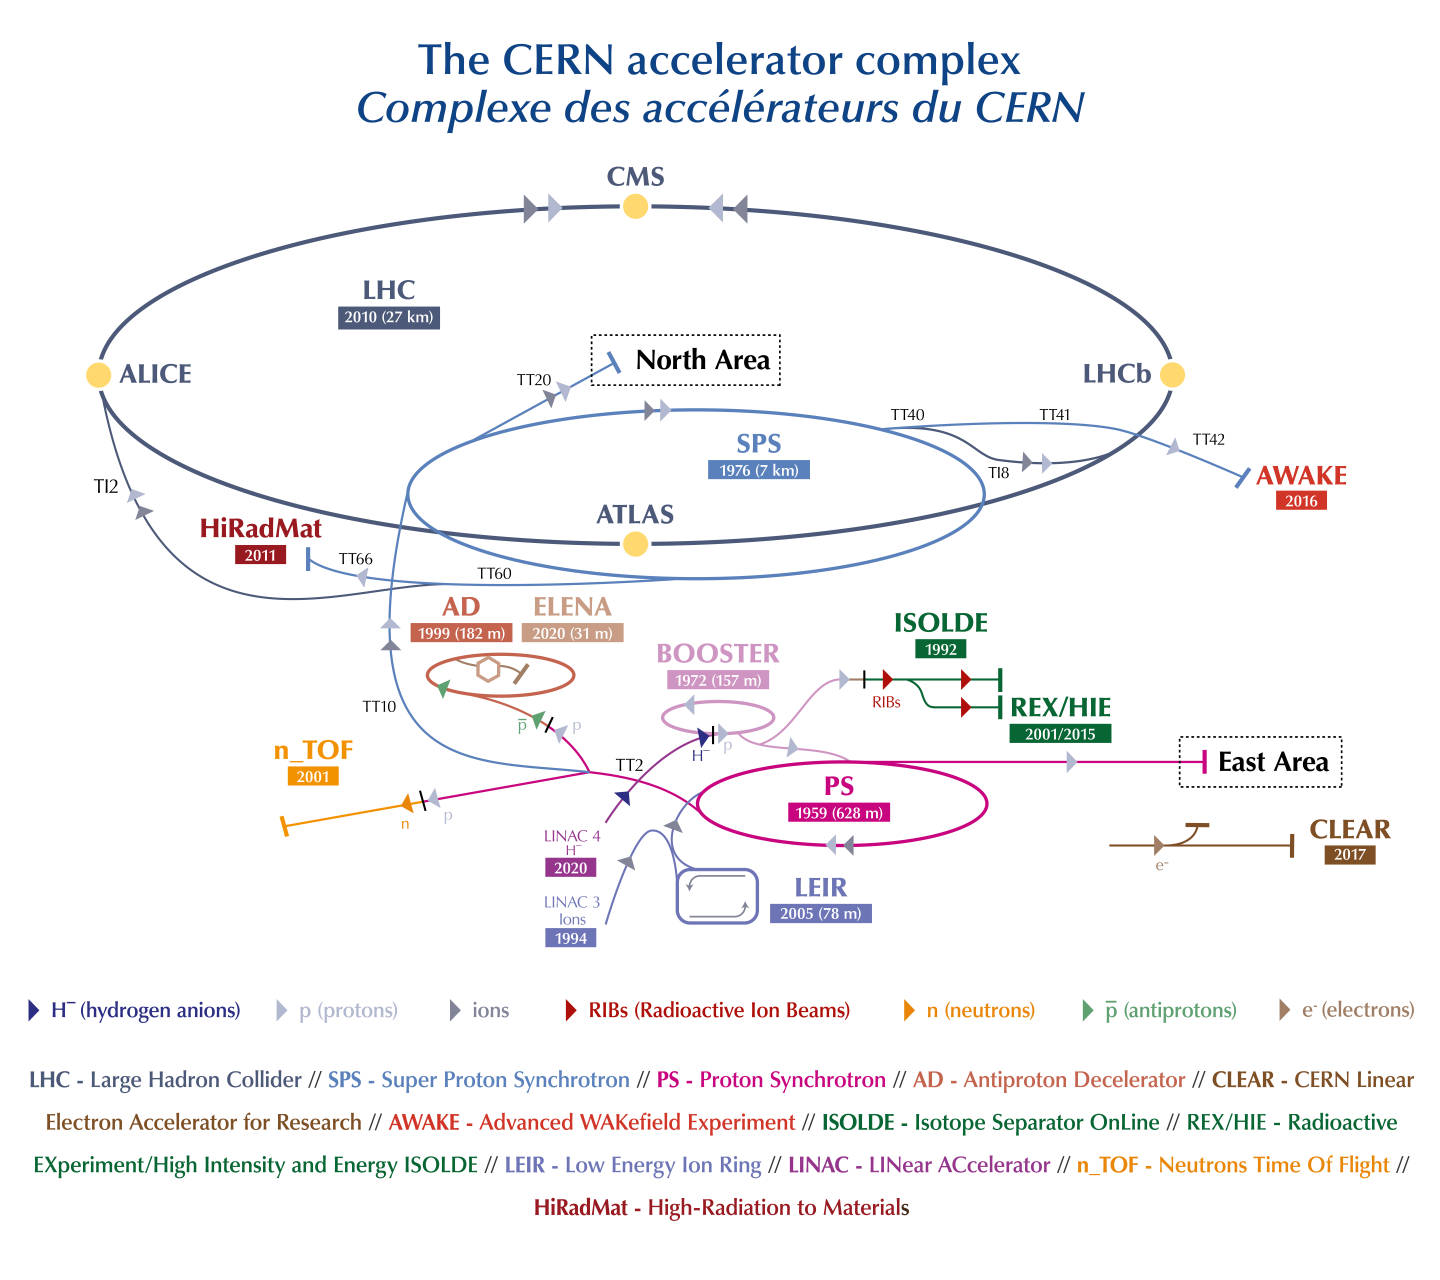
\includegraphics[width=4.5 in]{Images/Chap2/CERN_acc_system.png}
    \caption{CERN accelerating system. Figure from Ref. \cite{CERN_AcceleratorComplex}.}
    \label{fig:LHCAtlas/LHC/CERN_acc_system}
\end{figure}

The Large Hadron Collider (LHC) at CERN, with its 27 kilometres ring \cite{LHCguide}, is the world largest particle accelerator. 
It has four major interaction points which host the major CERN's experiments: ATLAS, CMS, LHCb and ALICE. 
LHC is situated around 100 metres underground to shield from radiation and for both economic\footnotemark and geological reasons. 
With its first run on 10 September 2008, it currently accelerates hadrons. Depending on the run, protons or lead nuclei are collided, with a center-of-mass energy of 13.6 TeV and 5.36 TeV respectively.
In order to reach such high energies, a complex system of pre-accelaration is adopted, as presented in Fig. \ref{fig:LHCAtlas/LHC/CERN_acc_system}.\\

\footnotetext{Building LHC on the surface would have required the purchase of properties to do so and an under the open sky structure with a 27 km circumference would have been more expensive than agreeing with landowner and excavate a tunnel underground.}


%-------------------------------------------------------------------------------

\subsection{CERN's accelerator system}\label{sec:LHCAtlas/LHC/CAS}

For proton-proton ($pp$) collisions, the process begins with the extraction of negative hydrogen ions ($H^-$), which are initially accelerated to an energy of $160\text{ MeV}$ by the Linear Accelerator 4 ($\text{LINAC4}$). 
Upon injection into the Proton Synchrotron Booster (PSB), the ions are stripped of their two electrons leaving only the bare protons, which are grouped into bunches and boosted to an energy of $2\text{ GeV}$. 
The protons then enter the Proton Synchrotron (PS), reaching an energy of $25\text{ GeV}$. 
The final step takes place in the Super Proton Synchrotron (SPS) that accelerates the proton bunches up to the LHC injection energy of $450\text{ GeV}$. 
Finally, the proton bunches are injected into the two counter-rotating beam pipes of the LHC, where they are accelerated to their maximum operational energy of $6.8\text{ TeV}$ per beam.\\
In heavy-ion operations (primarily based on lead nuclei, $^{208}\text{Pb}$), ions are initially accelerated by the Linear Accelerator 3 ($\text{LINAC3}$) to an energy of $4.2\text{ MeV per nucleon}$.
The nucleons are then accumulated and boosted to $72\text{ MeV per nucleon}$ inside the Low Energy Ion Ring (LEIR).
In the next stage, the PS accelerates ions to $5.9\text{ GeV per nucleon}$, before transferring them to the SPS where they reach an energy of $177\text{ GeV per nucleon}$. 
When injected into the main LHC ring, the heavy-ion beams are accelerated to a final energy of $2.68\text{ TeV per nucleon}$.\\
Particles are accelerated up to such high energies by means of radio-frequency (RF) cavities, resonant structures generating an oscillating electric field, with a fixed frequency of 400MHz, which accelerates charged particles each time they pass through. 
Particles with the target energy passing trough the cavity while the field is zero, will not be accelerated, while more (less) energetic particles will be decelerated (accelerated). 
Using this technique, it is ensured that particles stays in the cited bunches.


%-------------------------------------------------------------------------------

\subsection{The LHC parameters}\label{sec:LHCAtlas/LHC/parameters}

The LHC is composed by two circular beam pipes, denominated Beam 1 and Beam 2. Inside them, two particle beams, composed by a maximum of 2808 bunches with approximately $1.15\times10^{11}$ protons per bunch and spaced by 25 ns, travel separately close to the speed of light in opposite direction.
There are eight Interaction Points (IPs) along the LHC ring, but only four of them are used for collisions, hosting the main LHC experiments: ATLAS at IP1, ALICE (A Large Ion Collider Experiment) at IP2, CMS (Compact Muon Solenoid) at IP5 and LHCb (LHC beauty) at IP8.
The beam pipes and the interaction points are presented in Fig. \ref{fig:LHCAtlas/LHC/parameters/BeamsCERN}.

\begin{figure}[ht!]
    \centering
    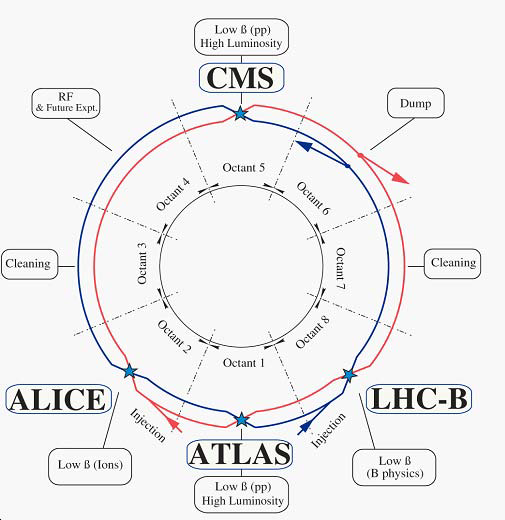
\includegraphics[width=2 in]{Images/Chap2/BeamsCERN.png}
    \caption{Schematic layout of the LHC (Beam 1 clockwise, Beam 2 anticlockwise). Figure from Ref. \cite{LHC_Machine}.}
    \label{fig:LHCAtlas/LHC/parameters/BeamsCERN}
\end{figure}

\noindent Due to the very high speed, when the two beams collide, the energy of the center of mass, known as $\sqrt{s}$, is twice the energy of each beam (which is the same). In fact, knowing that $E^2=m^2c^4+p^2c^2$ and using the natural unit system ([m]=eV/$c^2$, [p]=eV/c), we get: $E^2=m^2+p^2\simeq p^2$, where at the end an ultra-relativistic particle (p>>m) was assumed. This information is used in the norm of the four-momentum of two colliding particles:

\begin{equation}\label{eq:LHCAtlas/LHC/parameters/centerofmasseq}
    \sqrt{s}=\sqrt{P_{\mu}P^{\mu}}=\sqrt{E_{tot}^2-|\Vec{p_{tot}}|^2}=\sqrt{(E_1+E_2)^2-|\Vec{p_1}-\Vec{p_2}|^2}\simeq 2 E
\end{equation}

\noindent where we assumed $E_1$ = $E_2$. The 6.8 TeV of energy reached by LHC protons confirm the assumption p>>m and it leads to the known value of $\sqrt{s}=13.6 \text{ TeV}$.\\
Accelerated beams are directed and curved by superconducting electromagnets with a magnetic field of up to 8.3 T \cite{LHC_magnets}: 1232 dipole magnets and 392 quadrupole magnets are used to mantain the beams focused. 
Magnets are kept at a temperature of 1.9 K to ensure a 11600 A electric current which is needed for the intense magnetic field. 
Despite thier essential contribution, magnets also represent one of the main limitations of this apparatus. 
In fact, from the Lorentz force equation $\Vec{F}=q(\Vec{E}+\Vec{v}\times \Vec{B})$, it is possible to get a connection between the external magnetic field $\Vec{B}$ (the one generated by superconducting magnets), the  momentum $p$ of the particle circulating inside the beams and its radius of curvature $R$, which is:
\begin{equation}\label{eq:LHCAtlas/LHC/parameters/pqBR}
    p[GeV] = 0.3B[T]R[m]
\end{equation}

\noindent It is evident from Eq. \ref{eq:LHCAtlas/LHC/parameters/pqBR} that, to keep a constant momentum $p$ of the particles circulating inside the beams, a higher magnetic field $B$ is required in case of reduction of the radius of curvature $R$. Unfortunately, current technologies set a limit to the magnetic field generated by a magnet, limiting also the minum dimension of an accelerator ring.

\noindent Performance of the LHC are evaluated based on an essential parameter: the instantaneous luminosity $\mathcal{L}$. It defines the number of collisions per $cm^2$ and per second produced in the collider and thus it is  measured in $cm^{-2}s^{-1}$. It is computed as follows \cite{LHCreport}:
\begin{equation}\label{eq:LHCAtlas/LHC/parameters/Luminosity}
    \mathcal{L}=\frac{N_b^2n_bf_{rev}\gamma}{4 \pi \epsilon_n \beta^*}F
\end{equation}

\noindent where: $N_b$ is the number of particles in a bunch, $n_b$ is the number of bunches in a beam, $\epsilon_n$ is the normalized transverse beam emittance, $\beta^*$ is the beta function at the collision point, $\gamma$ is the Lorentz relativistic factor computed as $\gamma=1/\sqrt{1-v^2/c^2}$ , $f_{rev}$ is the revolution frequency. 
There is a connection between the beta function and the transverse beam size $\sigma$, which is $\sigma=\sqrt{\epsilon_n\beta^*/\gamma}$.
F represents the geometric luminosity reduction factor:
\begin{equation}
    F=\frac{1}{\sqrt{1+\Big(\frac{\theta_c\sigma_z}{2\sigma^*}\Big)^2}}
\end{equation}
\noindent where $\theta_c$ is the full crossing angle at the interaction point, $\sigma_z$ is the RMS bunch length and $\sigma^*$ is the transverse RMS beam size at the interaction point.
If during operations the instantaneous luminosity goes below a fixed threshold, beams are dumped and a new fill of the LHC is performed.\\
During LHC Run 3, $\mathcal{L}$ gets the value of $10^{34} \text{ cm}^{-2}s^{-1}$ for both ATLAS and CMS experiments, while for LHCb and ALICE it is $10^{32} \text{ cm}^{-2}s^{-1}$ and $10^{27} \text{ cm}^{-2}s^{-1}$ respectively.\\
The instantaneous luminosity is linked with the number of collisions per second :
\begin{equation}\label{eq:dNdt}
    \frac{dN}{dt}=\mathcal{L}\sigma_{tot}
\end{equation}
\noindent where $\sigma_{tot}$ is the total cross section, which is the measure of the probability of a specific interaction process to happen.
If the instantaneous luminosity is integrated over time, the number of events collected is obtained:
\begin{equation}\label{eq:LHCAtlas/LHC/parameters/Nevents}
    N_{events}=\sigma_{tot}\int \mathcal{L} dt 
\end{equation}

%-------------------------------------------------------------------------------

\subsection{LHC Run Schedule}

The LHC operations are structured into extended physics data-taking campaigns named \textit{Runs}, which are separated by planned technical maintenance and machine upgrade periods, which are known as Long Shutdowns (LS). 
It was Run 1, from 2010 to 2013, that started the LHC physics program, operating at center-of-mass energies of $\sqrt{s} = 7\text{ TeV}$ and $8\text{ TeV}$, with a delivered integrated luminosity of 28 $fb^{-1}$. Run 1 culminated in the discovery of the Higgs boson by the ATLAS and CMS collaborations.
Following upgrades during LS1, meant to enable higher-energy operations, Run 2 took place between 2015 and 2018 at $\sqrt{s} = 13\text{ TeV}$, delivering an integrated luminosity of approximately $156\text{ fb}^{-1}$.
After another round of upgrades during LS2 the collider entered the Run 3 era in 2022, which lasted until June 2026, operating at an increased center-of-mass energy of $\sqrt{s} = 13.6\text{ TeV}$. After having delivered an integrated luminosity of approximately $351\text{ fb}^{-1}$, the LHC was turned off for the begin of LS3.
This new stop will be used to prepare the LHC for the High-Luminosity LHC (HL-LHC) era, which is expected to start in 2029 and will last until 2042. The HL-LHC will operate at the same center-of-mass energy of Run 3 and is expected to deliver an integrated luminosity of $3000\text{ fb}^{-1}$ during the future Runs.\\
A graph showing the LHC delivered integrated luminosity during the different Runs, together with the recorded luminosity by ATLAS, is shown in Fig. \ref{fig:LHCAtlas/LHC/parameters/LumiATLAS}.

\begin{figure}[ht!]
    \centering
    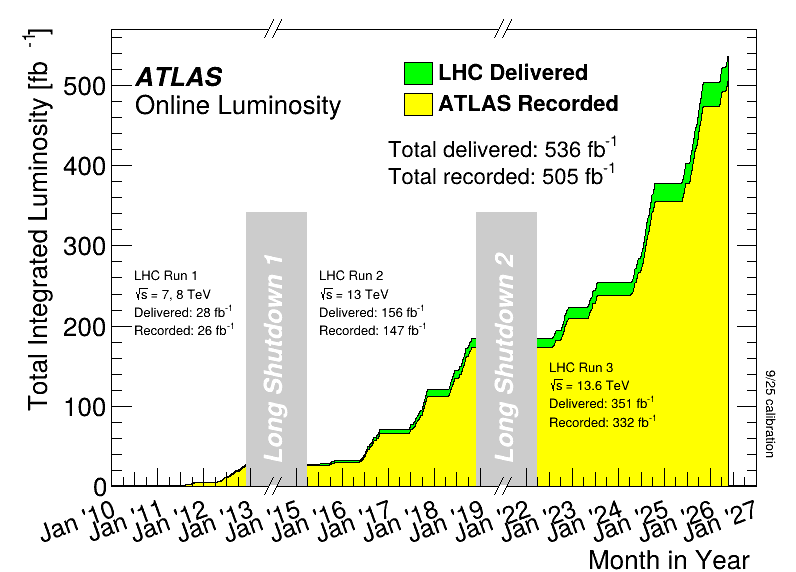
\includegraphics[width=3.5 in]{Images/Chap2/ATLAS_L_R1_R3.png}
    \caption{Cumulative integrated luminosity delivered to and recorded by the ATLAS Experiment during LHC Run 1, 2 and 3. Figure from Ref. \cite{ATLAS_Luminosity}.}
    \label{fig:LHCAtlas/LHC/parameters/LumiATLAS}
\end{figure}

%-------------------------------------------------------------------------------
%-------------------------------------------------------------------------------
\section{The ATLAS detector} \label{sec:LHCAtlas/ATLAS}

A Toroidal LHC ApparatuS (ATLAS) \cite{ATLASwebsite} is the world largest particle detector, situated at Interaction Point 1 at CERN.
44m in length and 25m in height are required to investigate collisions between particles accelerated by the LHC, to study phenomena such dark matter, the Higgs boson and top quark.
The ATLAS detector is composed by multiple sub-detectors organized in layers with a cylindrical symmetry around the beam pipe.
Among the main sub-detectors we can find: the Inner Detector (ID), the Electromagnetic Calorimeter (ECAL), the Hadronic Calorimeter (HCAL) and the Muon Spectrometer (MS), as shown in Fig. \ref{fig:LHCAtlas/ATLAS/ATLASdetector}.\\

\begin{figure}
    \centering
    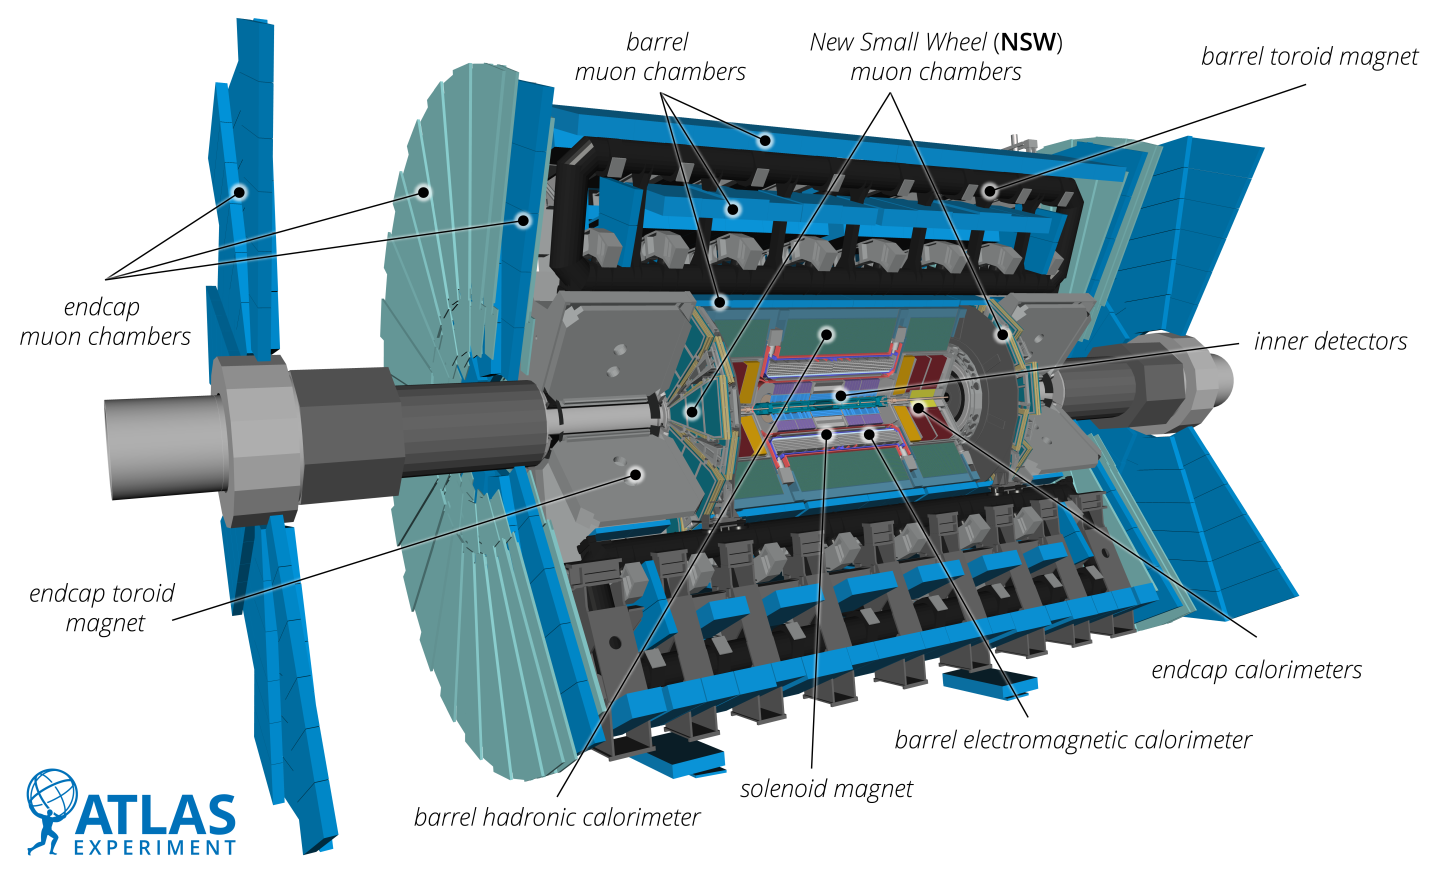
\includegraphics[width=4.3 in]{Images/Chap2/ATLASDetector.png}
    \caption{ATLAS schematic. Figure form Ref. \cite{ATLAS_detector}.}
    \label{fig:LHCAtlas/ATLAS/ATLASdetector}
\end{figure}

%-------------------------------------------------------------------------------
\subsection{Coordinate system} \label{sec:LHCAtlas/ATLAS/coordinatesystem}

Before analysing the ATLAS detector, it is important to introduce the coordinate system used to describe the position of particles and their momenta inside the sub-detectors. In figure \ref{fig:LHCAtlas/ATLAS/coordinatesystem/CoordinateSystem} an overview of the system is presented.

\begin{figure}[h!]
    \centering
    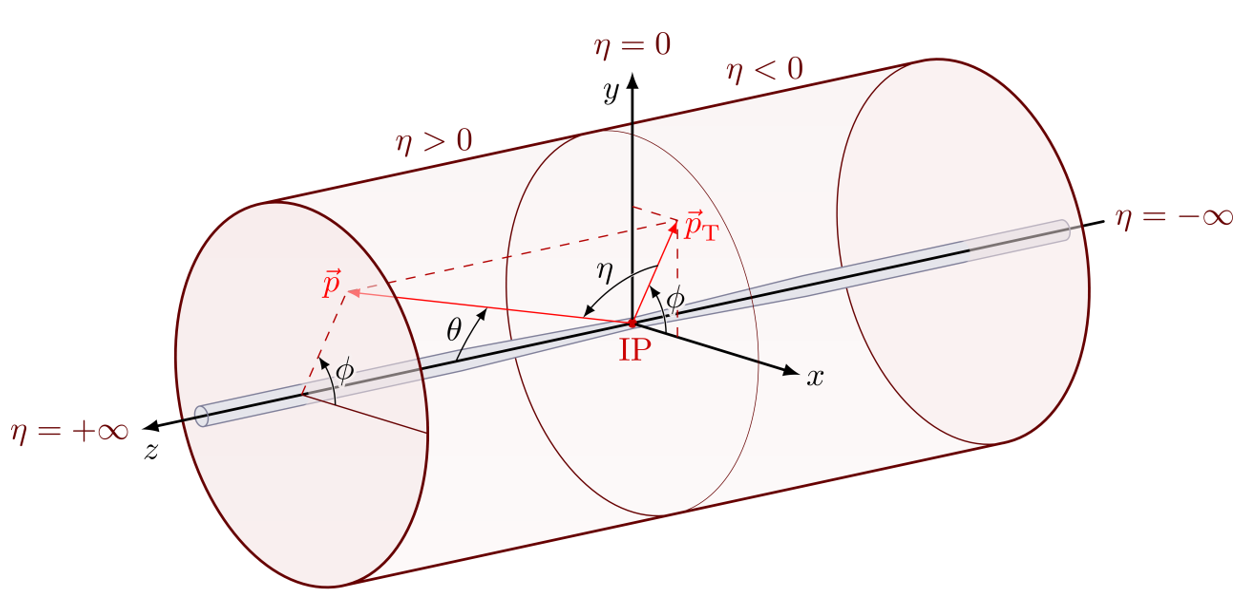
\includegraphics[width=3 in]{Images/Chap2/CoordinateSyst.png}
    \caption{Schematic of ATLAS coordinate system}
    \label{fig:LHCAtlas/ATLAS/coordinatesystem/CoordinateSystem}
\end{figure}

\noindent Cartesian axes (\textit{x,y,z}) are constructed as follows. The origin is set in the interaction point (IP). From it, the z-axis departs parallel to the beam tunnel with positive z-values in anticlockwise direction. As direct consequence, the x-y plane is perpendicular to it, with positive x-values towards the center of the LHC and positive y-values upward. On this Cartesian system, a cylindrical coordinate system ($r , \eta ,  \phi $) is defined to describe geometric position and components of particle momenta. $\phi$ is the azimuth angle, measured around the z-axis, with values [$-\pi , \pi $]. $\eta$ is named pseudo-rapidity and it is linked to the polar angle $\theta$ by the equation below:

\begin{equation}\label{eq:eta}
    \eta = - ln \Big( tan \frac{\theta}{2}\Big)
\end{equation}

\noindent The pseudo-rapidity and the azimuth angle, known as geographical coordinates \cite{ATLASexp}, are used to define a geometrical distance, applied when computing the separation between two physics objects:

\begin{equation} \label{eq:distance}
    \Delta R=\sqrt{\Delta \eta ^2 + \Delta \phi ^2}
\end{equation}

\noindent The third coordinate, $r$, is the radius from the center of the system. Actually, in this thesis, we use another information: the transverse momentum $p_T$. It is a 2D vector defined as the projection of the momentum in the transverse plane of the interaction. This parameter is related to the radius and it is important because it brings information about energy. In figure \ref{fig:pT} it is possible to observe how $p_T$ is calculated.


% \begin{figure}[h!]
%     \centering
%     \includegraphics[width=3 in]{Images/Cap4/TransverseMomentum.png}
%     \caption{Schematic of $p_T$ computing in the CMS experiment, analogous  to ATLAS}
%     \label{fig:pT}
% \end{figure}




The inner detector relies on a 2 T solenoidal magnetic field, parallel to the beam axis, to 
reconstruct the tracks of charged particles. This information is used to measure the momentum of them using the sagitta method and the relation between momentum and radius of curvature, presented in (\ref{eq:pqBR}).\\
The electromagnetic calorimeter \cite{ATLAS_detector} measures the energy of electrons, photons and hadrons. Once a particle among them hits the detector, an electromagnetic shower is generated and the energy of the particle is transferred to the material through radiation, as shown in figure \ref{fig:EMShower}. Passive components of the calorimeter such as lead induce the loss of energy and the active ones, made by Liquid Argon (LAr) kept at a temperature of -184 °C, measure it. The shower is fully contained in this part of the detector, which is longer then 20 radiation lengths. For this reason this technique to measure energy is defined \textit{destructive}.\\

% \begin{figure}[h!]
%     \centering
%     \includegraphics[width=3 in]{Images/Cap2/EMShower.png}
%     \caption{Schematic of an electromagnetic shower starting from a photon}
%     \label{fig:EMShower}
% \end{figure}

\noindent The hadronic calorimeter has been placed to measure the energy of hadrons that survive to the electromagnetic calorimeter. It relies on the principle of particle shower, which is converted into an electric current and measured.\\
The muon spectrometer is the last component of the ATLAS experiment and measures the momenta of muons. In fact, they are similar to electrons, but with a greater mass, which leads only to weak interactions and more depth of penetration. This is why they are not revealed by inner systems.\\
The coordinate system adopted at ATLAS to describe events is discussed in detail in section \ref{sec:CoordinateSystem}.

\chapter{Anomaly Detection} \label{chap:AD}

\section{The LHC} \label{sec:AD/AD}
\chapter{Anomaly Detection} \label{chap:AD}

As previously discussed in Sec. \ref{sec:SM_BSM/BSM}, SM is not a complete theory and New Physics beyond it should exist.
The usual model-dependent searches for BSM physics rely on MC simulations generated for specific BSM hypotheses to define signal-enriched regions.
They provide optimized sensitivity for the specific process although they remain blind to a broader scenario and they have not yet produced any significant discoveries.
This motivates the exploration of alternative approaches.\\
\textit{Model-independent searches} are the most common solution, as they do not rely on specific theoretical assumptions \cite{LHCOlympics}. 
They have been used for a long time among the High Energy Physics (HEP) community to derive limits on the production cross-section of BSM signals. 
Despite their name, these searches were still too dependent on the theoretical assumptions or on the simulation for the event selection and the background modelling, limiting their power.
Beyond that, their sensitivity was limited by the look-elsewhere effect \cite{LEE_HEP}.\\
Anomaly Detection (AD) addresses these constraints by identifying rare patterns without assuming a explicit signal hypotheses.

\section{Overview of Anomaly Detection}
\label{sec:ad_overview}

Anomaly Detection encompasses algorithms that identify data instances deviating significantly from nominal distributions \cite{belis2023machine, tinari2024}. 
In standard industrial contexts, anomalies manifest as out-of-sample or off-manifold events, such as fraudulent transactions or equipment failures \cite{kasieczka2021lhc, tinari2024}. 
In High Energy Physics (HEP), single events rarely provide statistical evidence of new phenomena; BSM signals typically manifest as subtle over-densities in phase space \cite{belis2023machine, kasieczka2021lhc}.

Within particle physics, ML-based AD strategies operate across different levels of supervision \cite{belis2023machine, tinari2024}. 
Weakly supervised methods, such as Classification Without Labels (CWoLa) and CATHODE, estimate localized over-densities by comparing signal-enriched regions against adjacent sidebands \cite{belis2023machine, tinari2024}. 
Conversely, fully unsupervised methods operate solely on background processes or unlabeled experimental data \cite{belis2023machine, tinari2024}. 
These algorithms isolate rare topology features in kinematic distributions, providing an unbiased tool for model-agnostic BSM searches \cite{belis2023machine, davide_proc}.

\section{Deep Learning and Neural Networks}\label{sec:dl_dnn}
Deep Learning (DL) models use stacked layers of parametrized mathematical transformations to extract abstract features from complex data inputs \cite{tinari2024, Russo_thesis}. 
A standard Deep Neural Network (DNN) processes an input vector $\mathbf{x} = (x_1, \dots, x_n)$ through hidden layers composed of individual processing units \cite{tinari2024, Russo_thesis}. 
The output $z$ of a single unit is defined as:\begin{equation}z = \sum_{i=1}^{n} w_i x_i + b\end{equation}where $w_i$ denotes trainable weights and $b$ represents the bias term \cite{tinari2024}. 
Non-linear activation functions $\sigma(z)$ map $z$ to break linear combinations across stacked layers \cite{tinari2024, Russo_thesis}:
\begin{equation}
y = \sigma(z)
\end{equation}
Common activation functions include the Rectified Linear Unit, $\text{ReLU}(z) = \max(0, z)$, and its smooth variant, the Gaussian Error Linear Unit \cite{tinari2024}:
\begin{equation}
    \text{GELU}(z) = z \cdot \Phi(z)
\end{equation}
where $\Phi(z)$ is the standard Gaussian cumulative distribution function \cite{tinari2024}. 
Network parameters update via gradient descent backpropagation, minimizing a task-specific loss function evaluating model predictions \cite{kasieczka2021lhc, tinari2024}.

\section{Graph Neural Networks}\label{sec:gnn}
Standard feedforward architectures struggle to process variable-size physical objects without imposing artificial ordering \cite{dav_ad_proc, Russo_thesis}. Hadronic jets, composed of varying counts of collimated sub-particles, naturally map to graph structures $G = (V, E)$, where $V$ denotes constituent nodes and $E$ represents interaction edges \cite{kasieczka2021lhc, davide_proc}. Node features contain kinematic variables $\mathbf{x}_i = (p_T, \eta, \phi)$, while edge features capture pairwise angular separations $\Delta R = \sqrt{(\Delta \eta)^2 + (\Delta \phi)^2}$ \cite{kasieczka2021lhc, davide_proc}.Graph Neural Networks (GNNs) preserve permutation invariance while executing local message passing \cite{kasieczka2021lhc, davide_proc}. The representation $\mathbf{h}_i^{(l)}$ of node $i$ at layer $l$ updates according to aggregated messages from its spatial neighborhood $\mathcal{N}(i)$ \cite{davide_proc}:\begin{equation}\mathbf{m}_{ij}^{(l)} = \phi_e \left( \mathbf{h}_i^{(l-1)}, \mathbf{h}j^{(l-1)}, \mathbf{e}{ij} \right)\end{equation}\begin{equation}\mathbf{h}i^{(l)} = \phi_v \left( \mathbf{h}i^{(l-1)}, \bigoplus{j \in \mathcal{N}(i)} \mathbf{m}{ij}^{(l)} \right)\end{equation}where $\phi_e$ and $\phi_v$ denote neural operations, $\mathbf{e}_{ij}$ is the edge feature, and $\bigoplus$ represents a permutation-invariant aggregation operator such as sum, mean, or max \cite{kasieczka2021lhc, davide_proc}. Graph-level outputs obtain global representations via permutation-invariant pooling functions across all nodes \cite{davide_proc}.

\section{Anomaly Detection Implementation via Deep Architectures}\label{sec:ad_implementation}
Unsupervised AD implementation utilizing DNNs and GNNs relies on latent representation learning \cite{belis2023machine, tinari2024}. Autoencoders (AEs) compress input graph representations $\mathbf{x}$ into a lower-dimensional bottleneck $\mathbf{z} = f_{\text{enc}}(\mathbf{x})$ before generating a reconstructed output $\hat{\mathbf{x}} = f_{\text{dec}}(\mathbf{z})$ \cite{belis2023machine, tinari2024}. When trained exclusively on dominant Standard Model background events, the network learns lossy compression tailored to nominal physics patterns \cite{belis2023machine, davide_proc}.Events containing BSM physics produce higher reconstruction errors due to unlearned substructure features \cite{belis2023machine, tinari2024}. An Anomaly Score ($AS$) is defined using the Mean Squared Error (MSE) metric \cite{belis2023machine, dav_ad_proc}:\begin{equation}AS = \frac{1}{N} \sum_{i=1}^{N} \left| \mathbf{x}_i - \hat{\mathbf{x}}_i \right|^2\end{equation}In ATLAS model-independent searches, cuts applied to the calculated $AS$ distribution isolate BSM candidates \cite{belis2023machine, davide_proc}. By filtering out high-probability background interactions, these architectures define signal-enriched regions directly from data, enabling model-agnostic resonance searches \cite{belis2023machine, tinari2024}.

% #################################################à
\section{What is it?}\label{sec:WhatisAD}
When applying Anomaly Detection \cite{DLforAD}\cite{LHCOlympics}, we are looking for outliers or rare events, which typically have a small deviation from already known events. In this case data is divided into two categories: "background", containing Standard Model events or noise, and "signal", including the hypothetical New Physics. All SM phenomena are classified within background without any distinction based on the origin of data. It is now possible to understand why Anomaly Detection is defined "model agnostic": in fact it does not rely on a specific theoretical model. This feature allows to scan a bigger range of events but it is less sensitive to any specific model. \\

% \begin{figure}[h!]
%     \centering
%     \includegraphics[width=2 in]{Images/Cap3/BumpHint.png}
%     \caption{Search for anomalies in particle physics. Figure from Ref. \cite{ML4ADHEP}}
%     \label{fig:bumphint}
% \end{figure}

\noindent To understand Anomaly Detection, we can use an example. Assuming we need to find a church in a town we do not know, without any technology. Instead of desperately walking around, we decide to climb an hill where we can scan the whole town with not so much effort. It is possible to identify the neighbourhood of the church or the "spatial region" where it is situated. We can also get some information we would not have got in the town, such as the colour of the roof or of the facade of the building we are looking for. Then we climb down the hill and go straight to the point we observed. Thanks to the details we obtained up there, we are able to find the church quite quickly and more easily. In other words, the church represents New Physics, climbing the hill is Anomaly Detection, climbing down is using normal data analysis techniques. It is quite powerful, isn't it? To apply Anomaly Detection it is necessary to hypothesize that anomalies are rare and they represent a small portion of a whole dataset. This assumption is realistic because it is what happens everyday in airports, finance and particle physics: normal events are way more common then deviations. In addition, if anomalies in Particle Physics were more frequent, we would have already observed them through common data analysis.

%%%%%%%%%%%%%%%%%%

\section{Deep Learning and Anomaly Detection}\label{sec:DLforAD}
While working on a Particle Physics problem, it is common to deal with a huge amount of data collected during collisions at the LHC. Machine Learning (ML) algorithms, which are able to learn from past by using vast datasets, can help in this sense. Among all categories of ML, Deep Learning (DL) is the best for our task \cite{LHCOlympics}. Based on a multi-layer Neural Network, DL can build complex data representation, which is optimal when dealing with high-dimensional dataset. Furthermore due to its implementation, that will be discussed in chapter \ref{chap:Model}, it can be exploited for model agnostic applications. \cite{ML4ADHEP}\\
ML and DL methods can be classified based on how the labels of data are used to train models. Main categories are: Supervised Learning, Unsupervised Learning and Semi-Supervised Learning.\cite{DLforAD}\\
In Supervised Learning, shown in figure \ref{fig:SUPtrain}, labeled data is used to train DL models and it can be implemented only with sufficient normal and anomalous data.

% \begin{figure}[h!]
%     \centering
%     \includegraphics[width=3.5 in]{Images/Cap3/SUPtraining.png}
%     \caption{Data used for Supervised Learning. Figure from Ref. \cite{DLforAD}}
%     \label{fig:SUPtrain}
% \end{figure}

\noindent Unsupervised Learning is based on not labeled data, as shown in figure \ref{fig:UNSUPtrain}, and models implementing it are trained to find a structure among the input features. Then model performance is tested using a mixed dataset containing both background and signal data.\\
Semi-Supervised Learning is a hybrid of previous techniques, implemented in the most varied ways.

% \begin{figure}[h!]
%     \centering
%     \includegraphics[width=2.7 in]{Images/Cap3/UNSUPtraining.png}
%     \caption{Data used for Unsupervised Learning. Figure from Ref. \cite{DLforAD}}
%     \label{fig:UNSUPtrain}
% \end{figure}

\noindent In this project we implemented an Unsupervised Anomaly Detection, because labels have not been used and model was trained only over background data.

%%%%%%%%%%%%%%%%%%%%%%
\section{How is it implemented?}\label{sec:ADimplementation}
The process of training a  DL model is divided into three main phases: training, validation and test loop. They are defined "loop" because in each of them a different section of the dataset is used and the code loops over it.\\
The most important stage is the training loop: in our case the chosen DL model is trained to reconstruct arrays containing information about particle jets, using only data with normal behaviour (background events) \cite{DLforAD}. In this phase, parameters of the model are adjusted in order to best fit to data. By doing so, DL model is able to recognise very well normal data and their structure. Our hope is that, once it faces an anomaly (signal event), it is able to identify it due to its difference from what it knows. The second step is the validation loop, where a valuation of the performance of the model is elaborated using the validation set. The valuation and the search for the best weights of the model are executed computing distance between output and input over training and validation set. When this distance is minimum within the validation loop, we save the model's weights.\\
The trained and tuned model is then tested, using a dataset containing unseen data, the test set, where there are both background and signal events. The purpose of this phase is to validate results previously obtained and get a preview of what will happen once the model will be running with completely new data. The task is completed computing the Anomaly Score (AS). In this thesis, we implement it as a distance between input and output, with different dimension: instead of calculating it over a batch of data, we do so for each event. In this way we are able to plot a reconstruction probability graph: we expect that the distributions of AS from background and signal events are different, because signal data contains anomalies which our model does not know. By means of these distributions we can identify a threshold of separation between them. For any event we pass to our trained model, we compute AS: if it higher (lower) than the chosen threshold, we are looking at a background (signal) event. Since AD is distinguishing signal events from background, we are basically executing a classification task with two classes. Implementation of Anomaly Detection is discussed more in depth in chapters \ref{chap:Model} and \ref{chap:Results}.

% \begin{figure}[h!]
%     \centering
%     \includegraphics[width=3 in]{Images/Cap3/ADtestloop.png}
%     \caption{Test loop of Anomaly Detection. Figure from Ref. \cite{DLforAD}}
%     \label{fig:RECOprob}
% \end{figure}



\chapter{ATLAS analysis with AD in hadronic final states} \label{chap:ADJJ}

The final and crucial chapter of this thesis is dedicated to present the implementation of the Anomaly Detection approach within an ATLAS analysis.
This study searches for boson resonances associated with BSM physics decaying into fully hadronic final states in the described detector, making use of the AD technique.\\
The goal of this analysis is to prove the feasibility of the AD approach in a full analysis, exploring its generalization capabilities, while hunting for New Physics and trying to improve the sensitivity of the search with respect to the state-of-the-art methods.\\ 
At the moment, the status of the analysis is the following.
The R\&D phase on the MC sample for the DNN model can be defined as concluded, as it is for the statistical analysis and modelling on the MC dataset.
The preparation of the field to move towards the usage of the real data is currently on going, expecting the switch in dataset to happen soon.\\
In the following sections, an overiew of the analysis is presented, with a description of the dataset and the Graph Neural Network model used for the AD implementation. 
After this, an important portion of the chapter is dedicated to the description of the original work related to this thesis, which is the execution of the statistical analysis on the MC dataset, with the aim of testing the AD approach in a full analysis.\\


%-------------------------------------------------------------------------------
%-------------------------------------------------------------------------------
\section{The dataset}\label{sec:ADJJ/dataset}
The analysis focuses on exploring the data collected by the ATLAS detector during the LHC Run-3 from 2022 to 2024.
It corresponds to a total integrated luminosity of 165 fb$^{-1}$, with a center-of-mass energy of $\sqrt{s} = 13.6$ TeV \cite{ATLAS_Luminosity}.\\
Before running the full analysis pipeline on the real data, a preliminary study is performed on a MC dataset, which is used to train and validate the AD model and to test the statistical tools developed.
The latter aspect is the goal of this thesis, which aims to conduct the analysis on the MC sample and validate the tools.
In this preliminary stage, a sample simluating 2023 events is used, the one developed during \textit{MC23d} campaign.\\
The composition of the dataset is described in the following.\\

%-------------------------------------------------------------------------------
\subsection{Final states}\label{sec:ADJJ/dataset/states}
This analysis hunts for BSM physics in the form of heavy resonances with masses in the TeV range which decay into quarks forming final states with two large-radius jets ($R=1.0$).
Such signatures are chosen because they are predicted by several NP models and they are characterized by a high Branching Ratio (BR), from which the analysis sensitivity could benefit.
Together with this, the high mass of the resonances results in highly boosted decay products, which are collimated and reconstructed as single large-radius jets each.
This leads to a final state where jets can present a complex substructure, which can be exploited by the AD model to identify possible anomalies and NP candidates.\\

\begin{figure}[ht!]
    \centering
    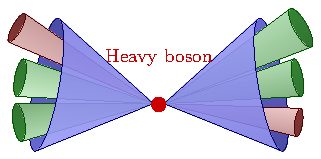
\includegraphics[width=2.5 in]{Images/Chap5/DecayingHeavyBoson.pdf}
    \caption{Schematic drawing of a heavy boson decaying into two large-radius jets (blue cones) with substructure, both normal (green cones) and anomalous (red cones).}
    \label{fig:ADJJ/dataset/states/HBdecay}
\end{figure}

%-------------------------------------------------------------------------------
\subsection{Signal processes}\label{sec:ADJJ/dataset/Signal}

Despite the model-agnostic nature of the AD approach, a set of benchmark signal processes has to be chosen to test the sensitivity of the technique.
In this analysis, two main physical processes are considered: Heavy Vector Triplet (Sec. \ref{sec:SM_BSM/BSM/HVT}) and Dark Jets (Sec. \ref{sec:SM_BSM/BSM/DJ}).\\
The Dark sector is probed using a sample of a $Z'$ boson with mass $m_{Z'} = 3.5 \text{ TeV}$, decaying into a pair of dark quarks with a mass $m_{q_D} = 20 \text{ GeV}$ each .\\
HVT, instead, are explored with three different processes.
The first one is the decay of a heavy vector boson $V$, assumed to be the candidate $Y$ boson, into a BSM vector boson $X$ and the SM Higgs boson $H$.
The masses of the $V$ and $X$ bosons are varied in order to explore different kinematic configurations, among $m_V = [2.3 , 3.4 , 5.0 , 6.0 ] \text{ TeV}$ and $m_X = [100 , 200, 2500, 400] \text{ GeV}$ respectively.
The mass of the Higgs boson, instead, is fixed to its SM value of $m_H = 125 \text{ GeV}$.\\
The second HVT process considered is the decay of a heavy vector boson $V$, into a pair of SM $W$ bosons.
Once again, the mass of the $V$ boson is varied among $m_V = [2.0 , 3.0 , 4.0 , 5.0 ] \text{ TeV}$, while the masses of the $W$ bosons are fixed to their SM value of $m_W = 80 \text{ GeV}$.\\
In conclusion, the third process studied is the decay of a heavy $W'$ boson into a $W$ and a $Z$ BSM bosons, with single masses at $m_{W'} = 3.0 \text{ TeV}$, $m_W = 200 \text{ GeV}$ and $m_Z = 400 \text{ GeV}$.\\
In all the three cases, bosons are assumed to decay into quarks, forming jets in the final state.\\
The complete list of signal processes considered in the analysis, together with their corresponding masses and theoretical cross-sections assumed, is reported in Tab. \ref{tab:sec:ADJJ/dataset/Signal}.
The theoretical cross-sections are derived from the ATLAS internal database for $MC23d$ campaign.

\begin{table}[htbp]
\raggedright
\begin{tabular}{|c|c||c||c|}
\hline
\rowcolor{lightgray}
\textbf{Signal Name} & \textbf{Process} & \textbf{Masses [GeV]} & \shortstack{\textbf{Theoretical}\\\textbf{cross-section [pb]}} \\
\hline\hline 

 VcXH & $V \to XH$ & $m_V = 2300$, $m_X = 100$ & $4.7435 \cdot 10^{-1}$ \\
 VcXH & $V \to XH$ & $m_V = 3400$, $m_X = 200$ & $4.1550 \cdot 10^{-2}$ \\
 VcXH & $V \to XH$ & $m_V = 5000$, $m_X = 2500$ & $1.6359 \cdot 10^{-3}$ \\
 VcXH & $V \to XH$ & $m_V = 6000$, $m_X = 400$ & $2.1811 \cdot 10^{-4}$ \\
\hline

 VzWW & $V \to WW$ & $m_V = 2000$ & $3.8476 \cdot 10^{-3}$ \\
 VzWW & $V \to WW$ & $m_V = 3000$ & $3.5969 \cdot 10^{-4}$ \\
 VzWW & $V \to WW$ & $m_V = 4000$ & $4.5256 \cdot 10^{-5}$ \\
 VzWW & $V \to WW$ & $m_V = 5000$ & $6.2648 \cdot 10^{-6}$ \\
\hline
 
 Wprime & $W' \to WZ$ & $m_{W'} = 3000$, $m_W = 200$, $m_Z = 400$ & $9.6982 \cdot 10^{-16}$ \\
\hline
 
 DarkJet & $Z' \to q_D \bar{q}_D$ & $m_{Z'} = 3500$, $m_{q_D} = 20$, $m_{q_D} = 20$ & $1.05853 \cdot 10^{-9}$ \\
\hline
 
\end{tabular}
\caption{Signal processes considered in the analysis, with their corresponding masses and theoretical cross-sections.}
\label{tab:sec:ADJJ/dataset/Signal}
\end{table}

%-------------------------------------------------------------------------------
\subsection{Background processes}\label{sec:ADJJ/dataset/BKG}


\begin{figure}[ht!]
    \centering
    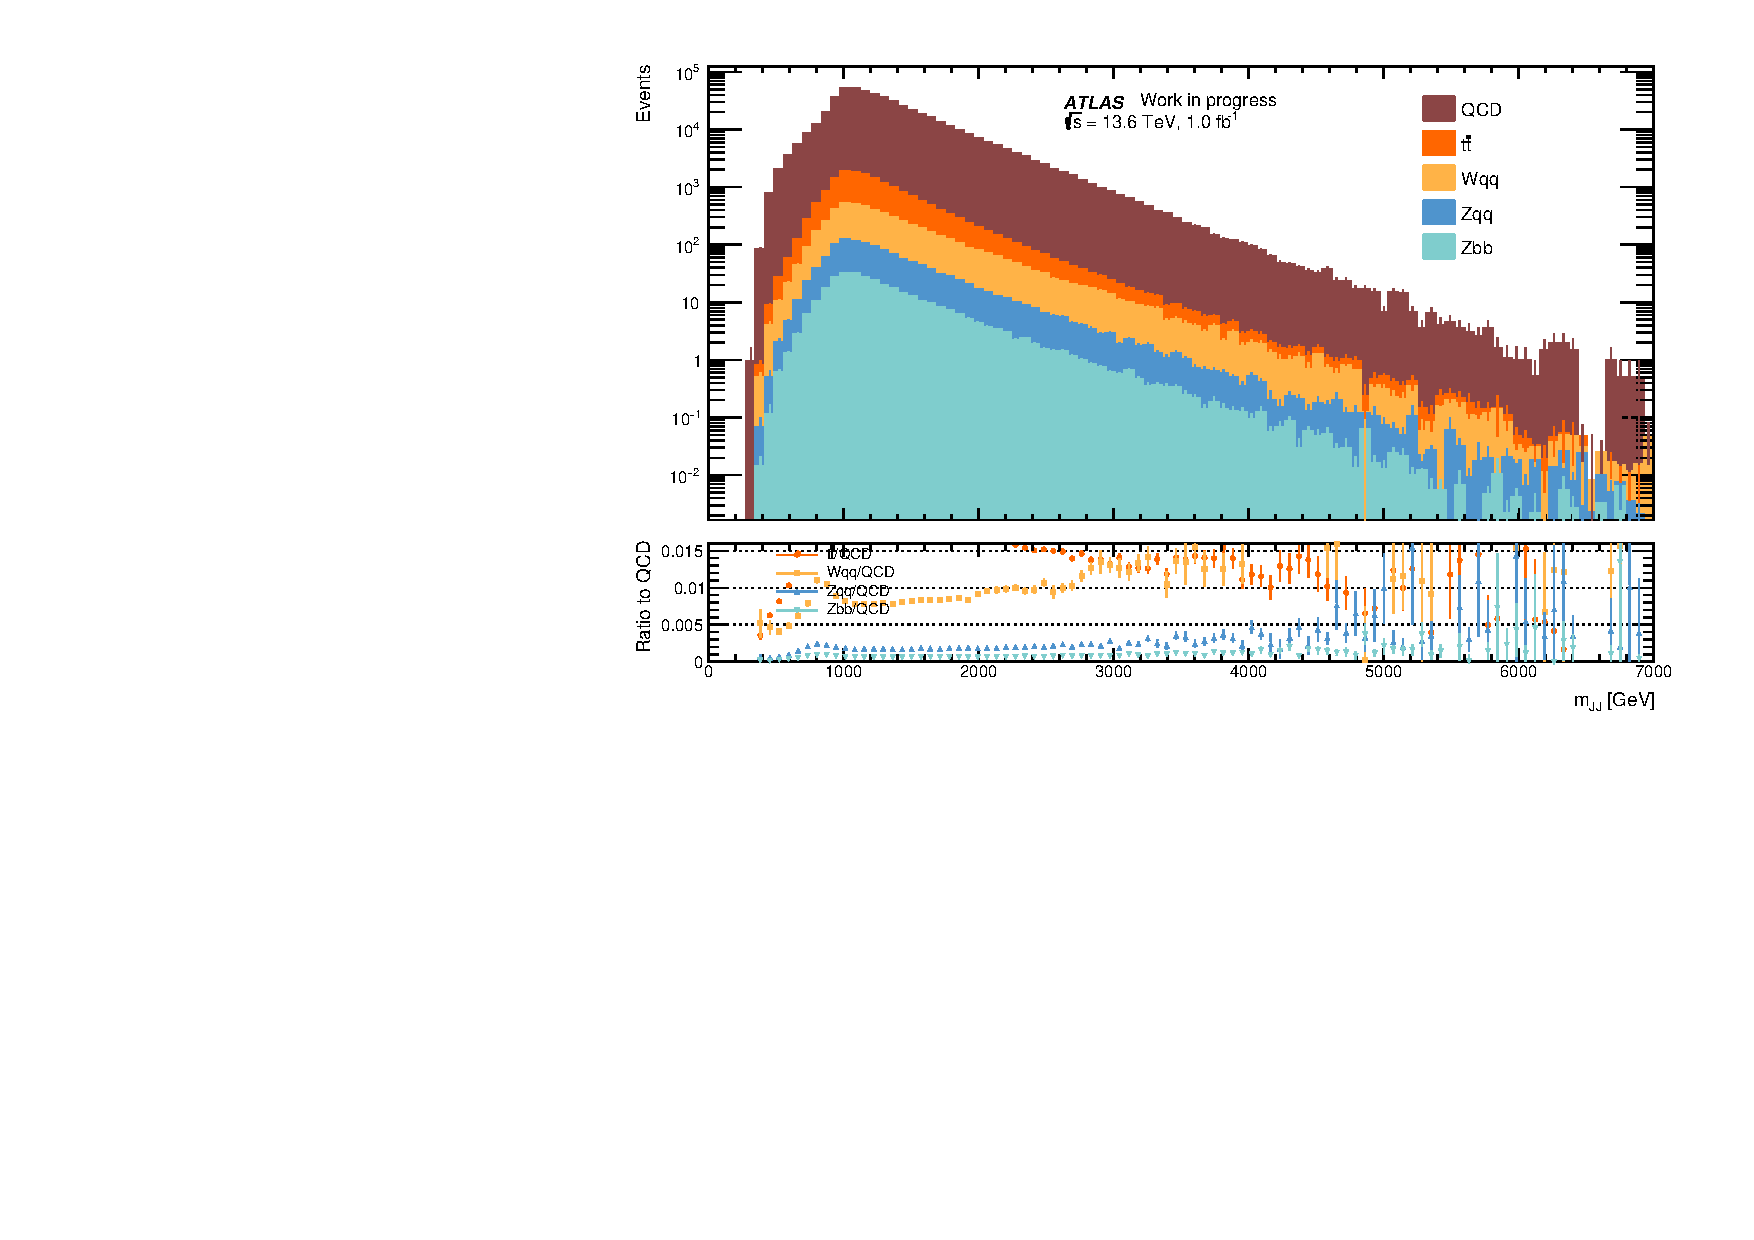
\includegraphics[width=4.5 in]{Images/Chap5/DataPlots/BKG_stack.pdf}
    \caption{Stacked distribution of the di-jet invariant mass $m_{JJ}$ for the dominant background processes considered in the analysis.}
    \label{fig:ADJJ/dataset/BKG/BKGstack}
\end{figure}

%-------------------------------------------------------------------------------
%-------------------------------------------------------------------------------
\section{Machine Learning }\label{sec:ADJJ/GNN}



%%%%%%%%%%%%%%%%%%%%%%%%%%%%%%%%%
%%%%%%%%%%%%%%%%%%%%%%%%%%%%%%%%%

\section{Graph Neural Networks}
\label{sec:gnn}

Particle physics events inherently feature variable numbers of reconstructed objects—such as tracks, topological clusters, or jet constituents—interacting within complex geometrical spaces. Graph Neural Networks (GNNs) exploit this structure by representing collision events as sparse directed graphs $G = (V, E)$, where nodes $v_i \in V$ correspond to individual particles or sub-detectors, and edges $e_{ij} \in E$ parameterize relational features or spatial separations $\Delta R = \sqrt{(\Delta\eta)^2 + (\Delta\phi)^2}$.

Node feature vectors $h_i^{(0)}$ encode basic spatial and kinematic observables, including transverse momentum $p_T$, pseudorapidity $\eta$, azimuthal angle $\phi$, and impact parameters. Graph neural architectures process relational topology through Message Passing Neural Network (MPNN) frameworks. At execution step $t$, node representations are updated iteratively using localized neighborhood information:
\begin{equation}
    m_i^{(t+1)} = \sum_{j \in \mathcal{N}(i)} \mathcal{M}_{\theta} \left( h_i^{(t)}, h_j^{(t)}, e_{ij} \right)
\end{equation}
\begin{equation}
    h_i^{(t+1)} = \mathcal{U}_{\phi} \left( h_i^{(t)}, m_i^{(t+1)} \right)
\end{equation}
where $\mathcal{N}(i)$ defines the set of immediate spatial neighbors of node $i$, $\mathcal{M}_{\theta}$ represents a parameterized message function, and $\mathcal{U}_{\phi}$ constitutes a node-state update function.

Permutation invariance across input node orderings is enforced via global pooling operations:
\begin{equation}
    h_G = \bigoplus_{v_i \in V} h_i^{(T)}
\end{equation}
where $\bigoplus$ represents a symmetric aggregation operator such as a element-wise summation, mean, or attention-weighted sum. In the context of large-radius jet substructure analyses within ATLAS, GNN architectures capture complex inter-particle correlations, color-flow dynamics, and energy distributions without relying on manually engineered substructure variables such as $N$-subjettiness $\tau_N$ or energy correlation functions $D_2$.

\section{Anomaly Detection Implementation with Deep Learning}
\label{sec:ad_implementation}

Deep-learning-based Anomaly Detection in High Energy Physics is operationalized through distinct architectural formulations:

\textbf{Self-Supervised Reconstruction Architectures:} Autoencoders (AEs) compress input vectors $x \in \mathbb{R}^d$ into a lower-dimensional latent representation $z \in \mathbb{R}^k$ ($k \ll d$) via an encoding network $f_\theta(x)$, subsequently reconstructing the input via a decoding network $g_\phi(z)$. Trained exclusively on dominant SM background events using loss metrics such as Mean Squared Error:
\begin{equation}
    \mathcal{L}_{\text{MSE}} = \| x - g_\phi(f_\theta(x)) \|^2
\end{equation}
the AE optimizes loss metrics for standard topologies. When evaluated on BSM topologies absent from training ensembles, the AE fails to accurately reconstruct the anomalous features, yielding significantly elevated reconstruction errors. These errors directly construct a continuous Anomaly Score (AS). Variational Autoencoders (VAEs) regularize this latent space by enforcing a standard Gaussian prior distribution $p(z) \sim \mathcal{N}(0, I)$ through a Kullback-Leibler divergence term $\mathcal{D}_{\text{KL}}$, balancing latent space continuity against reconstruction fidelity.

\textbf{Weakly-Supervised Overdensity Estimation:} The Classification Without Labels (CWoLa) paradigm isolates overdensities in resonant spectra by establishing mixed signal-plus-background datasets. Defining a Signal Region (SR) in a invariant mass continuum $m_{JJ}$ alongside adjacent Control Sidebands (SB), a classifier is trained directly on unlabeled experimental data to distinguish SR events from SB events. By the Neyman-Pearson Lemma, a classifier trained on mixed ensembles with differing signal proportions converges monotonically to the optimal Likelihood Ratio:
\begin{equation}
    R(x) = \frac{p_{\text{data}}(x | m \in \text{SR})}{p_{\text{bg}}(x | m \in \text{SR})}
\end{equation}

Advanced weakly-supervised density estimators, such as CATHODE, CURTAINS, and ANODE, employ conditional normalizing flows or optimal transport algorithms to model sideband background dynamics, interpolating background probability densities directly into the SR to eliminate feature correlations and artificial mass sculpting.

In the ATLAS ADJJ (Anomaly Detection in Dijet final states) analysis, GNN architectures are interfaced directly with model-independent search frameworks. Unsupervised GNN autoencoders process the constituent point-clouds of large-radius anti-$k_t$ ($R=1.0$) jets, outputting an Anomaly Score for every event. Selecting thresholds on the AS distribution defines specific Working Points (WPs), achieving background rejection factors spanning orders of magnitude. 

Model-independent signal searches are subsequently executed by scanning the di-jet invariant mass $m_{JJ}$ spectrum across defined AS WPs. Smooth parametric functions model the suppressed SM background background continuum, while potential anomalous signals are evaluated using flexible resonance fits, such as Double-Sided Crystal Ball functions. Binned maximum likelihood fits combined with the $\text{CL}_s$ statistical method derive 95\% Confidence Level upper limits on production cross-sections, providing a sensitivity bridge between deep graph representations and model-agnostic BSM discoveries at CERN.



%%%%%%%%%%%%%%%%%%%%%%%%%%%%%%%%%%
\section{Overview of Anomaly Detection}
\label{sec:ad_overview}

Anomaly Detection encompasses algorithms that identify data instances deviating significantly from nominal distributions \cite{belis2023machine, tinari2024}. 
In standard industrial contexts, anomalies manifest as out-of-sample or off-manifold events, such as fraudulent transactions or equipment failures \cite{kasieczka2021lhc, tinari2024}. 
In High Energy Physics (HEP), single events rarely provide statistical evidence of new phenomena; BSM signals typically manifest as subtle over-densities in phase space \cite{belis2023machine, kasieczka2021lhc}.

Within particle physics, ML-based AD strategies operate across different levels of supervision \cite{belis2023machine, tinari2024}. 
Weakly supervised methods, such as Classification Without Labels (CWoLa) and CATHODE, estimate localized over-densities by comparing signal-enriched regions against adjacent sidebands \cite{belis2023machine, tinari2024}. 
Conversely, fully unsupervised methods operate solely on background processes or unlabeled experimental data \cite{belis2023machine, tinari2024}. 
These algorithms isolate rare topology features in kinematic distributions, providing an unbiased tool for model-agnostic BSM searches \cite{belis2023machine, davide_proc}.


\section{Graph Neural Networks}\label{sec:gnn}
Standard feedforward architectures struggle to process variable-size physical objects without imposing artificial ordering \cite{dav_ad_proc, Russo_thesis}. Hadronic jets, composed of varying counts of collimated sub-particles, naturally map to graph structures $G = (V, E)$, where $V$ denotes constituent nodes and $E$ represents interaction edges \cite{kasieczka2021lhc, davide_proc}. Node features contain kinematic variables $\mathbf{x}_i = (p_T, \eta, \phi)$, while edge features capture pairwise angular separations $\Delta R = \sqrt{(\Delta \eta)^2 + (\Delta \phi)^2}$ \cite{kasieczka2021lhc, davide_proc}.Graph Neural Networks (GNNs) preserve permutation invariance while executing local message passing \cite{kasieczka2021lhc, davide_proc}. The representation $\mathbf{h}_i^{(l)}$ of node $i$ at layer $l$ updates according to aggregated messages from its spatial neighborhood $\mathcal{N}(i)$ \cite{davide_proc}:\begin{equation}\mathbf{m}_{ij}^{(l)} = \phi_e \left( \mathbf{h}_i^{(l-1)}, \mathbf{h}j^{(l-1)}, \mathbf{e}{ij} \right)\end{equation}\begin{equation}\mathbf{h}i^{(l)} = \phi_v \left( \mathbf{h}i^{(l-1)}, \bigoplus{j \in \mathcal{N}(i)} \mathbf{m}{ij}^{(l)} \right)\end{equation}where $\phi_e$ and $\phi_v$ denote neural operations, $\mathbf{e}_{ij}$ is the edge feature, and $\bigoplus$ represents a permutation-invariant aggregation operator such as sum, mean, or max \cite{kasieczka2021lhc, davide_proc}. Graph-level outputs obtain global representations via permutation-invariant pooling functions across all nodes \cite{davide_proc}.

\section{Anomaly Detection Implementation via Deep Architectures}\label{sec:ad_implementation}
Unsupervised AD implementation utilizing DNNs and GNNs relies on latent representation learning \cite{belis2023machine, tinari2024}. Autoencoders (AEs) compress input graph representations $\mathbf{x}$ into a lower-dimensional bottleneck $\mathbf{z} = f_{\text{enc}}(\mathbf{x})$ before generating a reconstructed output $\hat{\mathbf{x}} = f_{\text{dec}}(\mathbf{z})$ \cite{belis2023machine, tinari2024}. When trained exclusively on dominant Standard Model background events, the network learns lossy compression tailored to nominal physics patterns \cite{belis2023machine, davide_proc}.Events containing BSM physics produce higher reconstruction errors due to unlearned substructure features \cite{belis2023machine, tinari2024}. An Anomaly Score ($AS$) is defined using the Mean Squared Error (MSE) metric \cite{belis2023machine, dav_ad_proc}:\begin{equation}AS = \frac{1}{N} \sum_{i=1}^{N} \left| \mathbf{x}_i - \hat{\mathbf{x}}_i \right|^2\end{equation}In ATLAS model-independent searches, cuts applied to the calculated $AS$ distribution isolate BSM candidates \cite{belis2023machine, davide_proc}. By filtering out high-probability background interactions, these architectures define signal-enriched regions directly from data, enabling model-agnostic resonance searches \cite{belis2023machine, tinari2024}.

% #################################################à
\section{CURCH}\label{sec:WhatisAD}


%%%%%%%%%%%%%%%%%%


%%%%%%%%%%%%%%%%%%%%%%
\section{How is it implemented?}\label{sec:ADimplementation}
The process of training a  DL model is divided into three main phases: training, validation and test loop. They are defined "loop" because in each of them a different section of the dataset is used and the code loops over it.\\
The most important stage is the training loop: in our case the chosen DL model is trained to reconstruct arrays containing information about particle jets, using only data with normal behaviour (background events) \cite{DLforAD}. In this phase, parameters of the model are adjusted in order to best fit to data. By doing so, DL model is able to recognise very well normal data and their structure. Our hope is that, once it faces an anomaly (signal event), it is able to identify it due to its difference from what it knows. The second step is the validation loop, where a valuation of the performance of the model is elaborated using the validation set. The valuation and the search for the best weights of the model are executed computing distance between output and input over training and validation set. When this distance is minimum within the validation loop, we save the model's weights.\\
The trained and tuned model is then tested, using a dataset containing unseen data, the test set, where there are both background and signal events. The purpose of this phase is to validate results previously obtained and get a preview of what will happen once the model will be running with completely new data. The task is completed computing the Anomaly Score (AS). In this thesis, we implement it as a distance between input and output, with different dimension: instead of calculating it over a batch of data, we do so for each event. In this way we are able to plot a reconstruction probability graph: we expect that the distributions of AS from background and signal events are different, because signal data contains anomalies which our model does not know. By means of these distributions we can identify a threshold of separation between them. For any event we pass to our trained model, we compute AS: if it higher (lower) than the chosen threshold, we are looking at a background (signal) event. Since AD is distinguishing signal events from background, we are basically executing a classification task with two classes. Implementation of Anomaly Detection is discussed more in depth in chapters \ref{chap:Model} and \ref{chap:Results}.

% \begin{figure}[h!]
%     \centering
%     \includegraphics[width=3 in]{Images/Cap3/ADtestloop.png}
%     \caption{Test loop of Anomaly Detection. Figure from Ref. \cite{DLforAD}}
%     \label{fig:RECOprob}
% \end{figure}


\chapter{Conclusions} \label{chap:concl}

\cite{PhDGRusso}

\backmatter
\cleardoublepage

\newpage
\phantomsection
\addcontentsline{toc}{chapter}{\bibname}
\bibliography{bibliography}


\appendix

\phantomsection
\appendix 
\chapter*{Appendix A}
\section*{Plots}

aasdasdasdsadsadasdas





%\begin{acknowledgments}
\chapter*{Acknowledgments}
Un sentito e caloroso ringraziamento per questo lavoro va ai miei relatori, il prof. Stefano Giagu, il dott. Valerio Ippolito e il dott. Giuliano Gustavino.
Mi avete guidato, meeting dopo meeting, nella realizzazione di questo progetto, insegnandomi come cercare la nuova fisica e, soprattutto, l'approccio giusto per farlo, con spirito critico e curiosità.
Le lunghe chiacchierate in saletta, tra un caffè e un pranzo riscaldato, a discutere di tutti i dettagli, che oggi sembrano piccoli o persino ovvi, ma che si sono rivelati essenziali per la mia formazione.
Non so ancora cosa mi riserverà il futuro, ma so che, se sarò un buon fisico e ricercatore, sarà anche grazie a voi.\\
In secondo luogo, vorrei ringraziare Luca, per tutti i momenti di confronto e di supporto. 
Spero di tornare ad indossare presto la maglia rossa con il numero 16.\\
Ringrazio anche tutti i ricercatori e le ricercatrici \textit{senior} del gruppo ATLAS di Roma 1, per avermi accolto e condiviso con me le vostre esperienze e conoscenze.\\
Concludo i ringraziamenti ATLAS con un pensiero speciale ai membri giovani della saletta, laureandi e dottorandi, per aver condiviso con me le lunghe ed interminabili giornate in dipartimento, rendendole più leggere, piacevoli e divertenti, tra dubbi e curiosità, seri e meno seri.\\

%%%%%%%%%%%% OLD %%%%%%%%%%%%%%
% Un sentito ringraziamento va ai miei relatori, il prof. Stefano Giagu e la dott.ssa Graziella Russo, per avermi guidato nella realizzazione di questo lavoro. Vorrei inoltre ringraziarli per avermi accolto in \textit{saletta} e fatto conoscere questa bella e stimolante realtà.\\
% Giunti alla conclusione di questa dissertazione, applicando l'operatore $\hat{T}$, vorrei ringraziare:\\
% l'Associazione Italiana Studenti di Fisica (e non Fegato), AISF, per avermi dimostrato che c'è anche un'altra via per vivere la Fisica, un po' meno canonica ma ugualmente affascinante;\\
% il Pie$\check{z}$o per avermi mostrato l'aspetto umano dell'università e per avermi sopportato nei terribili periodi di sessione; \\
% Alessandro e Francesco, perché sono sufficienti tre birre e il solito bar per parlare di tutto e rendere i momenti difficili un brutto ricordo;\\ 
% il gruppo di Sanda Mareje, per essere stati parte viva della mia adolescenza e, oggi che siamo all'università, ogni volta che torniamo a Vasto, basta un messaggio per ritrovarci e sentirmi nuovamente a casa;\\
% Ale, che conosco da quando si frequentava lezione con un grembiule blu, con il quale ho condiviso tutti i principali eventi fino ad oggi, belli o meno, grazie della pazienza;
% la mia famiglia, per esserci stati nei momenti di difficoltà ed aver condiviso insieme momenti di festa.
% Infine, vorrei ringraziare i miei genitori, perché questo traguardo è anche vostro. Non deve essere facile vedere l'unico figlio partire di casa a 19 anni, direzione la capitale, con tanti sogni e paure. Non deve essere facile fare scelte e sacrifici per far vivere un giovane fuorisede. Non è stato facile, ma non mi avete fatto mancare mai il vostro supporto, fisicamente con la presenza di persona ed emotivamente, spronandomi a raggiungere vette sempre più alte. Grazie.\\
% Per concludere, vorrei riportare le parole che una persona cara mi aveva riferito in un'intervista. Alla mia domanda "Quale messaggio daresti ai giovani di oggi?" lui, rivolto a noi giovani, disse: "Ritrovate il colloquio e il dialogo con le persone. Ricominciate a guardare negli occhi chi vi circonda. Vi accorgerete che potrebbero esserci persone che condividono le vostre stesse passioni e voglia di costruire qualcosa di positivo. Fate le cose per passione e non tanto per farle."
%\end{acknowledgments}

\end{document}